\documentclass{article}
\usepackage[utf8]{inputenx}
\usepackage[margin=1in]{geometry}
\usepackage{amsmath, textcomp, amssymb, caption, subcaption}

\renewcommand{\Re}{\mathrm{Re}}
\renewcommand{\Im}{\mathrm{Im}}

\usepackage[RPvoltages]{circuitikz} % package used for drawing some circuits

\usepackage{xcolor} % Required for specifying colors by name
\definecolor{marinho}{RGB}{0, 100, 150} % defining an ocean-blue(ish) color 

\usepackage{tikz, tkz-euclide, pgfplots}
\usetikzlibrary{shapes, patterns, positioning, shapes.gates.logic.US}

% setting up symbols for vectors 'leaving' and 'entering' the screen.
\tikzset{
	% leaving
	odot/.style={
		circle,
		inner sep=0pt,
		node contents={$\odot$},
		scale=2
	}, %
	% entering
	otimes/.style={
		circle,
		inner sep=0pt,
		node contents={$\otimes$},
		scale=2
	} %
} %

\pgfplotsset{compat=newest}

\pgfplotsset{soldot/.style={color=green,only marks,mark=*}}
\pgfplotsset{holdot/.style={color=black,only marks,mark=*}}

\pgfplotsset{reddot/.style={color = red, only marks, mark=*}}
\pgfplotsset{bluedot/.style={color=blue, only marks, mark=*}}
\pgfplotsset{graydot/.style={color=gray!40, only marks, mark=*}}

\newcommand{\ihat}{\hat{\imath}}
\newcommand{\jhat}{\hat{\jmath}}
\newcommand{\khat}{\hat{k}}

\begin{document}

	%%%%%%%%%%%%%%%%%%%%%%%%%%%%%%%%%%%%%%%%%%%%%%%%%%%%%%%%%%%%%%%%%%%%%%%%%%%%%%%%%%%%%%%
									% free body diagrams %
	%%%%%%%%%%%%%%%%%%%%%%%%%%%%%%%%%%%%%%%%%%%%%%%%%%%%%%%%%%%%%%%%%%%%%%%%%%%%%%%%%%%%%%%
	
	% free body diagrams of tables fixed to the xz plane
	\begin{figure}[h!]\centering
		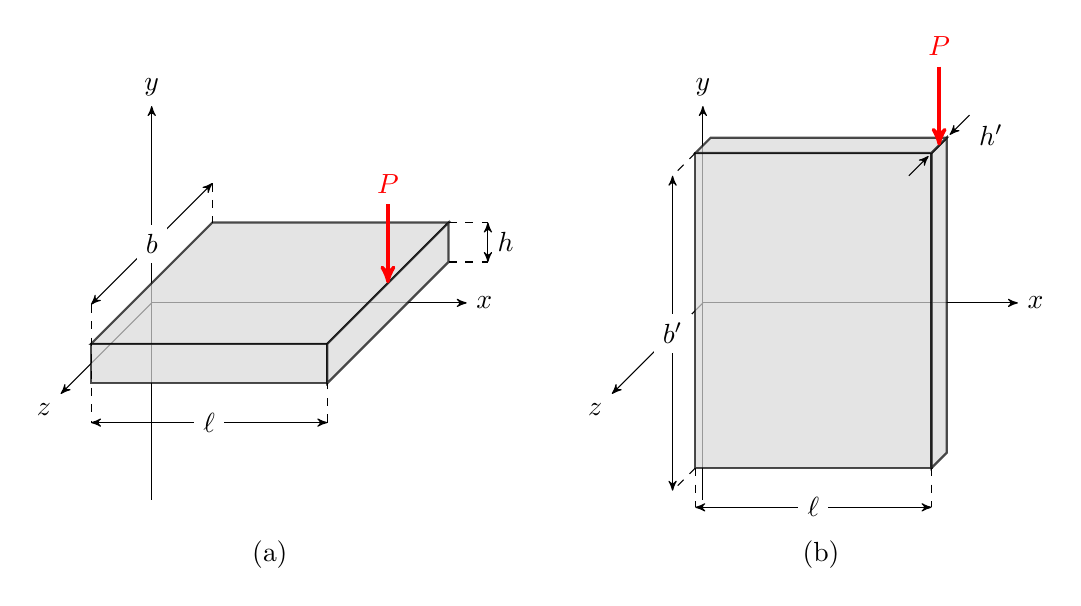
\begin{tikzpicture}[> = stealth']
			\draw [->] (0,0,0) -- (4,0,0) node [right] {$x$};
			\draw [->] (0,-2.5,0) -- (0,2.5,0) node [above] {$y$};
			\draw [->] (0,0,0) -- (0,0,3) node [below left] {$z$};
			
			%% ``Paralelepípedo''
			\draw [thick, fill=gray!30, opacity=0.7] 
			(0,0.25,-2) -- (3,0.25,-2) -- (3,0.25,2) -- (0,0.25,2) -- cycle;
			
			\draw [thick, fill=gray!30, opacity=0.7] 
			(0,0.25,2) -- (3,0.25,2) --(3,-0.25,2) -- (0,-0.25,2) -- cycle;
			
			\draw [thick, fill=gray!30, opacity=0.7]
			(3,0.25,2) --(3,-0.25,2) -- (3,-0.25,-2) -- (3,0.25,-2) -- cycle;
			
			%% Medidas
			\draw [<->] (0, -0.75, 2) -- (3, -0.75, 2) node [midway, fill=white] {$\ell$};
			\draw [<->] (0,0.75, 2) -- (0,0.75,-2) node [midway, fill=white] {$b$};
			\draw [dashed] (0,0.75,-2) -- (0,0.25,-2);
			\draw [dashed] (3,-0.75,2) -- (3,-0.25,2);
			\draw [dashed] (0,0.75, 2) -- (0,-0.75, 2);
			
			\draw [<->] (3.5,-0.25,-2) -- (3.5,0.25,-2) node [midway, right] {$h$};
			\draw [dashed] (3,-0.25,-2) -- (3.5,-0.25,-2);
			\draw [dashed] (3, 0.25,-2) -- (3.5, 0.25,-2);
			
			%% P
			\draw [->, red, very thick] (3,1.25,0) --++ (0,-1) node [at start, above] {$P$}; 
			
			%% (a)
			\node at (1.5, -3.2, 0) {(a)};
			
			\begin{scope}[shift={(7,0)}]
				\draw [->] (0,0,0) -- (4,0,0) node [right] {$x$};
				\draw [->] (0,-2.5,0) -- (0,2.5,0) node [above] {$y$};
				\draw [->] (0,0,0) -- (0,0,3) node [below left] {$z$};
				
				%% ``Paralelepípedo''
				\draw [thick, fill=gray!30, opacity=0.7] 
				(0,2,0.25) -- (0,-2,0.25) -- (3,-2,0.25) -- (3,2,0.25) -- cycle;
				
				\draw [thick, fill=gray!30, opacity=0.7] 
				(3,-2,0.25) -- (3,-2,-0.25) -- (3,2,-0.25) -- (3,2,0.25) -- cycle;
				
				\draw [thick, fill=gray!30, opacity=0.7]
				(3,2,0.25) -- (0,2,0.25) -- (0,2,-0.25) -- (3,2,-0.25) -- cycle; 				
				
				%% Medidas
				\draw [<->] (0,-2.5,0.25) -- (3,-2.5,0.25) node [midway, fill=white] {$\ell$};
				\draw [dashed] (0,-2, 0.25) -- (0,-2.5, 0.25);
				\draw [dashed] (3,-2, 0.25) -- (3,-2.5, 0.25);
				
				\draw [<->] (0,-2,1) -- (0,2,1) node [midway, fill=white] {$b'$};
				\draw [dashed] (0,2,0.25) -- (0,2,1);
				\draw [dashed] (0,-2,0.25) -- (0,-2,1);
				
				\draw [->] (3,2,1) -- (3,2,0.35);
				\draw [->] (3,2,-1) -- (3,2,-0.35) node [at start, below right] {$h'$};
				
				%% P
				\draw [->, red, very thick] (3,3,0) --++(0,-1) node [at start, above] {$P$};
				
				%% (b)	
				\node at (1.5, -3.2, 0) {(b)};
			\end{scope}
		\end{tikzpicture}
	\end{figure} % 
	
	% free body diagram of a disk pinned at O
	\begin{figure}[h!]\centering
		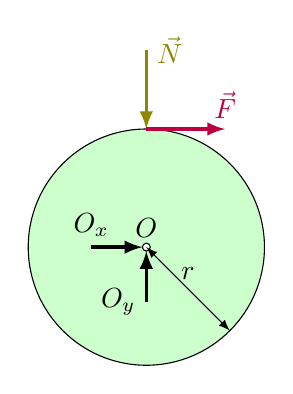
\begin{tikzpicture}
			%% Roda
			\draw[fill=green!20] (0,0) circle [radius=1.5cm];
			\draw[fill=white] (0,0) circle [radius=0.05cm];
				
			%% O
			\coordinate[label=above: $O$] (O) at (0,0);
				
			%% r
			\draw[latex-latex] (O)--(1.06,-1.06)
			node [midway, above] {$r´$};
				
			%% N
			\draw[-latex, olive, very thick] (0,2.5)--(0,1.5)
			node [at start, right] {$\vec{N}$};
				
			%% F
			\draw[-latex, purple, very thick] (0,1.5)--(1,1.5)
			node [at end, above] {$\vec{F}$};
				
			%% Ox, Oy
			\draw[-latex, very thick] (-0.7,0)--(-0.05,0)
				 node [at start, above] {$O_x$};
			\draw[-latex, very thick] (0,-0.7,0)--(0,-0.05)
			     node [at start, left] {$O_y$};				
		\end{tikzpicture}
	\end{figure} %
	
	% free body diagram of a ladder (there is no friction at B)
	\begin{figure}[h!]\centering
		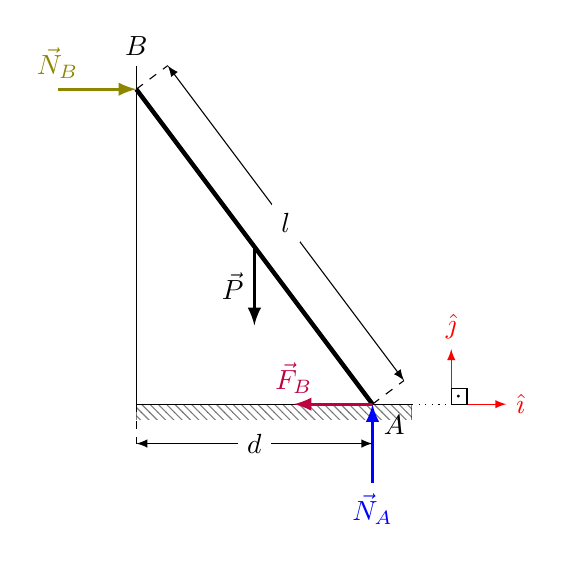
\begin{tikzpicture}
			%% barra, parede, chão
			\draw (3.5,0)--(0,0)--(0,4.3)
			node [at end, above] {$B$};
			\draw[ultra thick] (0,4)--(3,0)
			node [at end, below right] {$A$};
			
			\draw[pattern=north west lines, opacity=0.5] 
			(0,-0.2)--(0,0)--(3.5,0)--(3.5,-0.2);
			
			%% P
			\draw[-latex, very thick] (1.5,2)--(1.5,1)
			node [midway, left] {$\vec{P}$};
			
			%% N_A
			\draw[blue, -latex, very thick] (3,-1)--(3,0)
			node [at start, below] {$\vec{N}_A$};
			
			%% N_B
			\draw[olive, -latex, very thick] (-1,4)--(0,4)
			node [at start, above] {$\vec{N}_B$};
			
			%% F_B
			\draw[purple, -latex, very thick] (3,0)--(2,0)
			node [at end, above] {$\vec{F}_B$}; 
			
			%% d
			\draw[dashed] (0,0)--(0,-0.5);
			\draw[latex-latex] (0,-0.5)--(3,-0.5)
			node [midway, fill=white] {$d$}; 
			
			%% l
			\draw[dashed] (0,4)--(0.4,4.3);
			\draw[dashed] (3,0)--(3.4,0.3);
			\draw[latex-latex] (0.4,4.3)--(3.4,0.3)
			node [midway, fill=white] {$l$};
			
			%% i, j
			\coordinate (O) at (4,0);
			\coordinate (X) at (4.7,0);
			\coordinate (Y) at (4,0.7);
			
			\draw[dotted] (3.5,0)--(O);
			\draw[-latex, red] (O)--(X) node [at end, right]
			{$\ihat$};
			\draw[-latex, red] (O)--(Y) node [at end, above]
			{$\jhat$};
			
			\tkzMarkRightAngle[size=0.2](Y,O,X);
			\tkzLabelAngle[dist=.13](X,O,Y){$\cdot$};
		\end{tikzpicture}
	\end{figure} %
	
	% free body diagram of an arm ABC
	\begin{figure}
		\centering 
		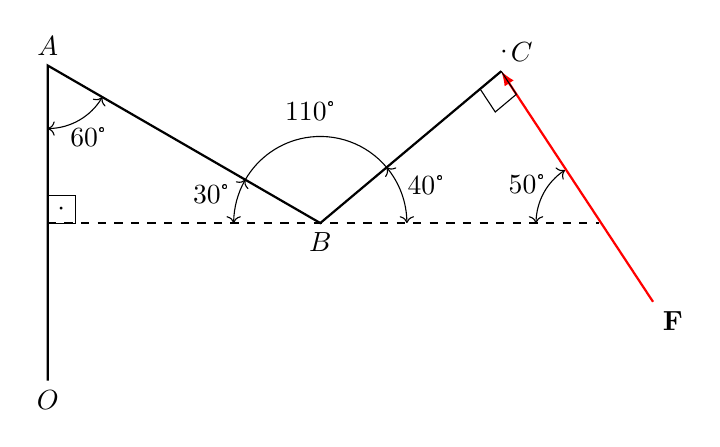
\begin{tikzpicture}
			\coordinate[label=below:$O$] (O) at (0,1);
			\coordinate[label=above:$A$] (A) at (0,5);
			\coordinate[label=below:$B$] (B) at (3.46,3);
			\coordinate[label=above right:$C$] (C) at (5.758,4.928);
			\coordinate (X) at (0,3);
			\coordinate (Y) at (7,3);
			\coordinate (Z) at (0,3);
			\coordinate[label=below right:$\mathbf{F}$] (F) at (7.686,2);
			
			\draw[thick] (O)--(A)--(B)--(C);
			\draw[dashed, thick] (X)--(Y);
			\draw[thick, -latex, red] (F)--(C);
			
			\draw pic["30\textdegree", draw=black, <->, angle eccentricity=1.3, angle radius=1.1cm]{angle=A--B--X}; 
			
			
			\draw pic["40\textdegree", draw=black, <->, angle eccentricity=1.3, angle radius=1.1cm]{angle=Y--B--C}; 
			
			\draw pic["50\textdegree", draw=black, <->, angle eccentricity=1.3, angle radius=0.8cm]{angle=C--Y--B};
			
			\draw pic["60\textdegree", draw=black, <->, angle eccentricity=1.3, angle radius=0.8cm]{angle=O--A--B};
			
			\draw pic["110\textdegree", draw=black, angle eccentricity=1.3, angle radius=1.1cm]{angle=C--B--A}; 
			
			\tkzMarkRightAngle[size=0.35](B,Z,A);
			\tkzLabelAngle[dist=.24](B,Z,A){$\cdot$};
			
			\tkzMarkRightAngle[size=0.35](F,C,B);
			\tkzLabelAngle[dist=.24](F,C,B){$\cdot$};
		\end{tikzpicture}
	\end{figure} %
	
	% free body diagram of a rope
	\begin{figure}[h!]
		\centering
		\begin{tikzpicture}[scale=0.8]
			% A, B, C e corda
			\coordinate[label=above right: \large{$A$}] (A) at (0,2);
			\coordinate[label=above: \large{$C$}] (C) at (2,-1);
			\coordinate[label=above left: \large{$B$}] (B) at (5,4);
			\draw plot [smooth, ultra thick] coordinates {(A) (C) (B)};	
			
			% TA
			\coordinate (P) at (-1,2);
			\coordinate (Q) at (1,-0.5);
			\coordinate (R) at (1,2);
			\coordinate (S) at (-1,4.5);
			
			\draw[dashed] (A)--(Q);
			\draw[dashed] (R)--(P);
			\draw[-latex, very thick] (A)--(S) node [at end, above left]{\large{$\mathbf{T_A}$}}; 	
			
			\draw pic["\large{$\theta$}", draw=black, angle eccentricity=1.3, angle radius=0.6cm]{angle=S--A--P};
			\draw pic["\large{$\theta$}", draw=black, angle eccentricity=1.3, angle radius=0.6cm]{angle=Q--A--R};
			
			% TB
			\coordinate (X) at (4,4);
			\coordinate (Y) at (6,4);
			\coordinate (Z) at (6,6);
			\coordinate (W) at (4,1.8);
			
			\draw[dashed] (X)--(Y);
			\draw[-latex, very thick] (B)--(Z) node [at end, above right]{\large{$\mathbf{T_B}$}};
			\draw[dashed] (B)--(W);
			
			\draw pic["\large{$\alpha$}", draw=black, angle eccentricity=1.4, angle radius=0.6cm]{angle=Y--B--Z};
			\draw pic["\large{$\alpha$}", draw=black, angle eccentricity=1.4, angle radius=0.6cm]{angle=X--B--W};
			
			% T
			\draw[-latex, very thick] (C)--(4,-1) node [at end, right]{\large{$\mathbf{T}$}};
			
			% P
			\draw[very thick, -latex] (C)--(2,-4) node [midway, right]{\large{$\mathbf{P}$}};
		\end{tikzpicture}
	\end{figure}%	
	
	% free body diagram of a fixed beam
	\begin{figure}[h!]\centering
		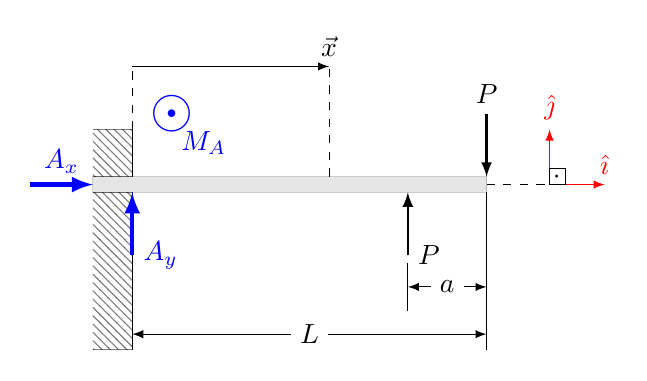
\begin{tikzpicture}
			% viga
			\draw[fill=gray, opacity=0.2] (0,0)--(0,0.2)--(5,0.2)--(5,0)--cycle;
			
			% engaste
			\draw (0.5,-2)--(0.5,0);
			\draw (0.5,0.2)--(0.5,0.8);
			\draw[pattern=north west lines, opacity=0.5] (0,0)--(0.5,0)--(0.5,-2)--(0,-2);
			\draw[pattern=north west lines, opacity=0.5] (0,0.2)--(0.5,0.2)--(0.5,0.8)--(0,0.8);
			
			% P's
			\draw[-latex, thick] (5,1)--(5,0.2) 
			node [at start, above] {$P$};
			\draw[-latex, thick] (4,-0.8)--(4,0) 
			node [at start, right] {$P$};
			
			% comprimentos
			\draw (5,0)--(5,-2);
			\draw (4,-0.9)--(4,-1.5);
			% a
			\draw[latex-latex] (4,-1.2)--(5,-1.2)
			node [midway, fill=white] {$a$};
			% L
			\draw[latex-latex] (0.5,-1.8)--(5,-1.8)
			node [midway, fill=white] {$L$};
			
			% esforçoes
			% Ay
			\draw[-latex, blue, ultra thick] (0.5,-0.8)--(0.5,0)
			node [at start, right] {$A_y$};
			% Ax
			\draw[-latex, blue, ultra thick] (-0.8,0.1)--(0,0.1)
			node [midway, above] {$A_x$};
			% M_A
			\node[odot, blue, at={(1,1)}];	
			\draw (1,0.9)--(1,0.9) node [blue, below right] {$M_A$};
			
			% vetor x
			\draw[dashed] (0.5,0.8)--(0.5,1.6);
			\draw[dashed] (3,0.2)--(3,1.6);
			\draw[-latex] (0.5,1.6)--(3,1.6)
			node [at end, above] {$\vec{x}$};
			
			% direções i, j
			\coordinate (O) at (5.8,0.1);
			\coordinate (i) at (6.5,0.1);
			\coordinate (j) at (5.8,0.8);
			
			\draw[dashed] (5,0.1)--(5.8,0.1);
			% i
			\draw[-latex, red] (O)--(i)
			node [at end, above] {$\ihat$};
			% j
			\draw[-latex, red] (O)--(j)
			node [at end, above] {$\jhat$};
			
			\tkzMarkRightAngle[size=0.2](i,O,j);
			\tkzLabelAngle[dist=.13](i,O,j){$\cdot$};
		\end{tikzpicture}
	\end{figure} %
	
	% free body diagram of a beam segment under generic stress distribution
	\begin{figure}[h!]\centering
		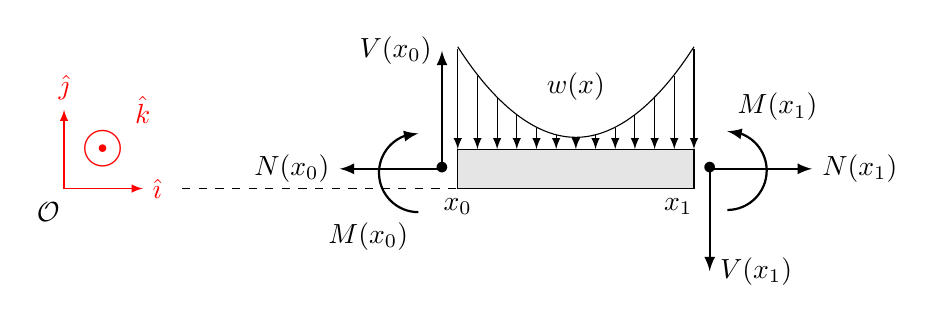
\begin{tikzpicture}
			%% i, j, k, A
			\draw [-latex, red] (-5, 0) -- (-4, 0) node [at end, right] {$\ihat$};
			\draw [-latex, red] (-5, 0) -- (-5, 1) node [at end, above] {$\jhat$};
			\node [odot, red, at={(-4.5, 0.5)}];
			\node [at={(-4, 1)}, red] {$\khat$}; 
			\node at (-5.2, -0.3) {$\mathcal{O}$};
			
			%% Comprimento de viga
			\draw [dashed] (-3.5, 0) -- (1,0);
			\draw [fill=gray!20] (0,0) -- (3,0) -- (3,1/2) -- (0,1/2) -- cycle
			node [at={(0,0)}, below] {$x_0$}
			node [at={(2.8,0)}, below] {$x_1$};		
			
			%% q, A_y, N, V, M, 
			%\draw [very thick, purple] (10,0) parabola bend (10.75,1) (12,-2);
			\draw (0,1.8) parabola bend (1.5, 0.65) (3, 1.8) node [at={(1.5,1)}, above] {$w(x)$};
			\foreach \i in {0, 0.25, ..., 3} {
				\draw [-latex] (\i, 0.5*\i*\i-1.5*\i+3.55*0.5) -- (\i,1/2);
			}
			
			\draw [thick, latex-] (-0.5, 0.7) arc (90:270:0.5) node [at end, below left]{$M(x_0)$};
			\draw [-latex, thick] (-0.2, 1/4) -- (-1.5, 1/4) node [at end, left] {$N(x_0)$}
			node [at start] {$\bullet$};
			\draw [-latex, thick] (-0.2, 1/4) -- (-0.2, 1.75) node [at end, left] {$V(x_0)$};
			
			\draw [thick, latex-] (12:3.5) arc (90:-90:0.5) node [at start, above right] {$M(x_1)$};
			\draw [-latex, thick] (3.2, 1/4) -- (4.5, 1/4) node [at end, right] {$N(x_1)$}
			node [at start] {$\bullet$};
			\draw [-latex, thick] (3.2, 1/4) -- (3.2, -1.05) node [at end, right] {$V(x_1)$};
		\end{tikzpicture}
	\end{figure} %	
	
	% free body diagram of a deformable body under twisting
	\begin{figure}[h!]\centering
		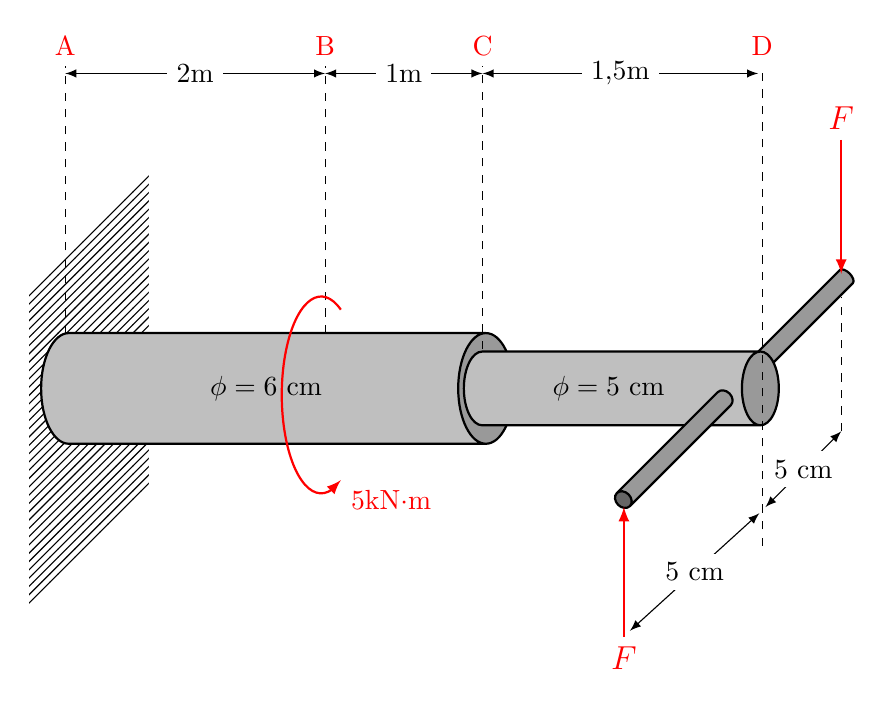
\begin{tikzpicture} [> = latex]
			\draw [color=white, pattern = north east lines]
			(-2,-2,2) -- (-2,-2,-2) -- (-2,2,-2) -- (-2,2,2) -- cycle;
			
			\node[thick, cylinder, draw, shape aspect=0.5,  
			cylinder uses custom fill, cylinder end fill=black!40, minimum height=1cm,
			cylinder body fill=black!25, scale=6]{};
			
			\begin{scope}[shift={(7,0.8)}]	
				\node[thick, cylinder, draw, shape aspect=0.5,  
				cylinder uses custom fill, cylinder end fill=black!60, minimum height=2cm,
				cylinder body fill=black!40, scale=1, rotate=225]{};	
			\end{scope}
			
			\begin{scope}[shift={(4.5,0)}]	
				\node[thick, cylinder, draw, shape aspect=0.5,  
				cylinder uses custom fill, cylinder end fill=black!40, minimum height=1cm,
				cylinder body fill=black!25, scale=4]{};	
			\end{scope}
			
			\begin{scope}[shift={(5.5,-0.7)}]	
				\node[thick, cylinder, draw, shape aspect=0.8,  
				cylinder uses custom fill, cylinder end fill=black!60, minimum height=2cm,
				cylinder body fill=black!40, scale=1, rotate=225]{};
			\end{scope}
			
			\draw [dashed] 
			(-2.3, 0.7,0) -- (-2.3, 4.1,0) node [at end, above, red] {A}
			(1, 0.7,0) -- (1,4.1,0) 	   node [at end, above, red] {B}
			(3, 0.5,0) -- (3, 4.1,0) 	   node [at end, above, red] {C}
			(6.55, -2,0) -- (6.55, 4.1,0)  node [at end, above, red] {D}
			(6.4, -1.7, -3) -- (6.4, 0, -3);
			
			\draw [thick, ->, red] (6.4, 2, -3) -- (6.4, 0.3, -3) 
			node [at start, above]  {\large{$F$}};
			
			\draw [thick, ->, red] (5.95,-2, 3) -- (5.95,-0.35,3) 
			node [at start, below] {\large{$F$}};
			
			\draw [<->] (6.4, -1.7, -0.3) -- (5.95, -2, 2.8) node [midway, fill=white] {5 cm};
			\draw [<->] (6.4, -1.7, -3) -- (6.4, -1.7, -0.5) node [midway, fill=white] {5 cm};
			
			\draw [<->] (-2.3, 4,0) -- (1,4,0) node [midway, fill=white] {2m};
			\draw [<->] (3, 4,0) -- (1,4,0) node [midway, fill=white] {1m};
			\draw [<->] (3, 4,0) -- (6.5,4,0) node [midway, fill=white] {1,5m};
			
			\node at (0.25,0,0) {$\phi=6$ cm};
			\node at (4.6,0,0) {$\phi=5$ cm};
			
			\draw [thick, red, ->] (1.2,1) arc (60:300: 0.5 and 1.25) 
			node [at end, below right] {5kN$\cdot$m};
		\end{tikzpicture}
	\end{figure} %

	% (simplified) free body diagram of a bike wheel's break.	
	\begin{figure}[h!]
		\centering
		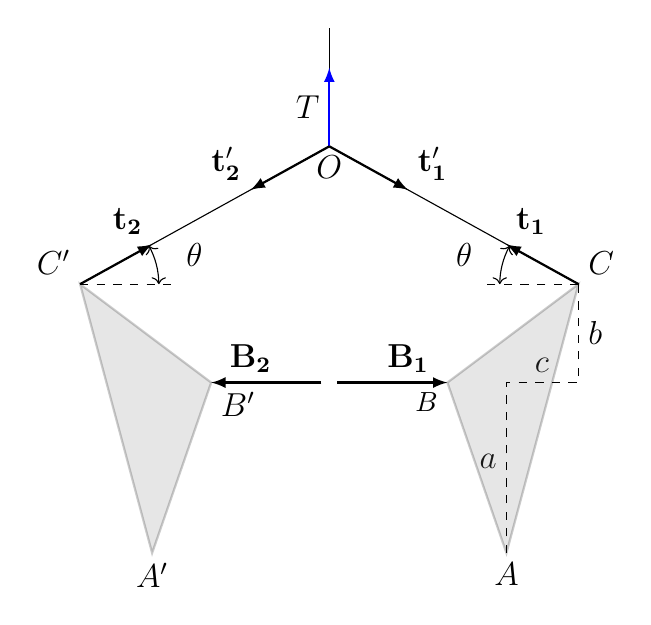
\begin{tikzpicture}[scale=0.5]		
			% B, A, C
			\coordinate[label=below left:$B$] (B) at (3,0);
			\coordinate[label=below:\large{$A$}] (A) at (4.5,-4.33);
			\coordinate[label=above right:\large{$C$}] (C) at (6.33,2.5);		
			
			% B', A', C'
			\coordinate[label=below right:\large{$B'$}] (B') at (-3,0);
			\coordinate[label=below:\large{$A'$}] (A') at (-4.5,-4.33);
			\coordinate[label=above left:\large{$C'$}] (C') at (-6.33,2.5);
			
			% O, T
			\coordinate[label=below:\large{$O$}] (O) at (0,6);
			\coordinate[label=left:\large{$T$}] (T) at (0,7);
			
			% a, b, c
			\coordinate[label=left:\large{$a$}] (a) at (4.5,-2);
			\coordinate[label=right:\large{$b$}] (b) at (6.33,1.25);
			\coordinate[label=above:\large{$c$}] (c) at (5.4,0);
			
			% B1, B2	
			\coordinate[label=above:\large{$\mathbf{B_1}$}] (B1) at (2,0);
			\coordinate[label=above:\large{$\mathbf{B_2}$}] (B2) at (-2,0);	
			
			% t1, t2		
			\coordinate[label=above right:\large{$\mathbf{t_1}$}] (t1) at (4.5,3.511);
			\coordinate[label=above left:\large{$\mathbf{t_2}$}] (t2) at (-4.5,3.511);
			
			% t1', t2'
			\coordinate[label=above right:\large{$\mathbf{t_1'}$}] (t1') at (2,4.894);
			\coordinate[label=above left:\large{$\mathbf{t_2'}$}] (t2') at (-2,4.894);
			
			\coordinate (X) at (-4,2.5);
			\coordinate (Y) at ( 4,2.5);
			
			% peças cinzas
			\draw[thick, fill=gray, opacity=0.2] (A) -- (B) -- (C) -- cycle;
			\draw[thick, fill=gray, opacity=0.2] (A') -- (B') -- (C') -- cycle;
			
			% fio
			\draw (C)--(O);
			\draw (C')--(O);
			\draw (O)--(0,9);
			
			% vetores B1, B2
			\draw[thick, -latex] (0.2,0)--(3,0);
			\draw[thick, -latex] (-0.2,0)--(-3,0);
			
			% vetor T
			\draw[thick, -latex, blue] (O)--(0,8);
			
			% vetores t1, t1'
			\draw[thick, -latex] (O)--(t1');
			\draw[thick, -latex] (C)--(t1);
			
			% vetor t2, t2'
			\draw[thick, -latex] (O)--(t2');		
			\draw[thick, -latex] (C')--(t2);
			
			% tracejado de a, b, c
			\draw[dashed] (A)--(4.5,0)--(6.33,0)--(C);
			
			% angulos
			% tracejado de auxílio
			\draw[dashed] (C')--(X);
			\draw[dashed] (C)--(Y);
			
			% thetas
			\draw pic["\large{$\theta$}", draw=black, <->, angle eccentricity=1.5, angle radius=1cm]{angle=X--C'--O};
			
			\draw pic["\large{$\theta$}", draw=black, <->, angle eccentricity=1.5, angle radius=1cm]{angle=O--C--Y};
		\end{tikzpicture}
	\end{figure} %
	
	% free body diagram of a fan's feet as seen from above.
	\begin{figure}
		\centering
		\begin{tikzpicture}
			% pernas
			\draw (-3,0)--(0,0);
			\draw (0,0)--(1.5,2.598);
			\draw (0,0)--(1.5,-2.598);
			
			% C
			\coordinate[label=above left:$C$] (C) at (0.1,0.1);
			
			% b
			\draw[dashed] (-3,0)--(-3,-0.5);
			\draw[dashed] (0,0)--(0,-0.5);
			\draw[latex-latex] (-3,-0.5)--(0,-0.5) node [midway,fill=white]{$b$};
			
			% B1, B2
			\node [odot,at={(1.5,2.598)}];
			\coordinate[label=above right:\large{$\mathbf{B_1}$}] (B1) at (1.6,2.698);
			\node [otimes,at={(1.5,-2.598)}];
			\coordinate[label=below right:\large{$\mathbf{B_2}$}] (B2) at (1.6,-2.698);
			
			% angulo
			\draw pic["120\textdegree", draw=black, <->, angle eccentricity=1.5, angle radius=1cm]{angle=B2--C--B1};
		\end{tikzpicture}
	\end{figure} %
	
	% free body diagram of a road sign.
	% here, F is the force applied by the wind
	\begin{figure}[h!]
		\centering
		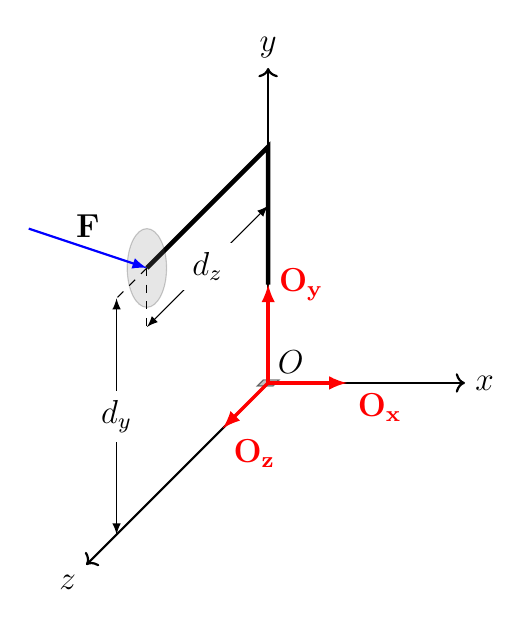
\begin{tikzpicture}[scale=0.5]
			% eixos e origem	
			\coordinate[label=above right:\large{$O$}] (O) at (0,0,0);	
			\draw[thick,->] (O) -- (5,0,0) node[at end, right]{\large{$x$}};
			\draw[thick,->] (O) -- (0,8,0) node[at end, above]{\large{$y$}};
			\draw[thick,->] (O) -- (0,0,12) node[at end, below left]{\large{$z$}};
			
			% placa
			\draw[ultra thick] (0,2.5,0)--(0,6,0)--(0,6,8);
			\draw[fill=gray, opacity=0.2] (0,6,8) ellipse (0.5cm and 1cm);
			
			% engaste
			\draw[fill=gray, opacity=0.5] (0.2,0,-0.2)--(-0.2,0,-0.2)--(-0.2,0,0.2)--(0.2,0,0.2)--cycle;
			
			% dy
			\draw[dashed] (0,6,8)--(0,4.5,8);
			\draw[latex-latex] (0,4.5,8)--(0,4.5,0) 
			node [midway, fill = white]{\large{$d_z$}};
			
			% dz
			\draw[dashed] (0,6,8)--(0,6,10);
			\draw[latex-latex] (0,6,10)--(0,0,10) node [midway, fill=white]{\large{$d_y$}};
			
			% F
			\draw[thick, blue, -latex] (-3,7,8)--(0,6,8) node [midway, above, black]{\large{$\mathbf{F}$}};
			
			%Ox, Oy, Oz	
			\draw[-latex, very thick, red] (O)--(2,0,0) node [at end, below right]{\large{$\mathbf{O_x}$}};
			\draw[-latex, very thick, red] (O)--(0,2.5,0) node [at end, right]{\large{$\mathbf{O_y}$}};	
			\draw[-latex, very thick, red] (O)--(0,0,3) node [at end, below right]{\large{$\mathbf{O_z}$}};			
		\end{tikzpicture}
	\end{figure} %
	

	%%%%%%%%%%%%%%%%%%%%%%%%%%%%%%%%%%%%%%%%%%%%%%%%%%%%%%%%%%%%%%%%%%%%%%%%%%%%%%%%%%%%%%%
								  % geometry constructions %
	%%%%%%%%%%%%%%%%%%%%%%%%%%%%%%%%%%%%%%%%%%%%%%%%%%%%%%%%%%%%%%%%%%%%%%%%%%%%%%%%%%%%%%%
	
	% steps for the construction of a regular pentagon (straightedge and compass only)
	\begin{figure}
		\centering
		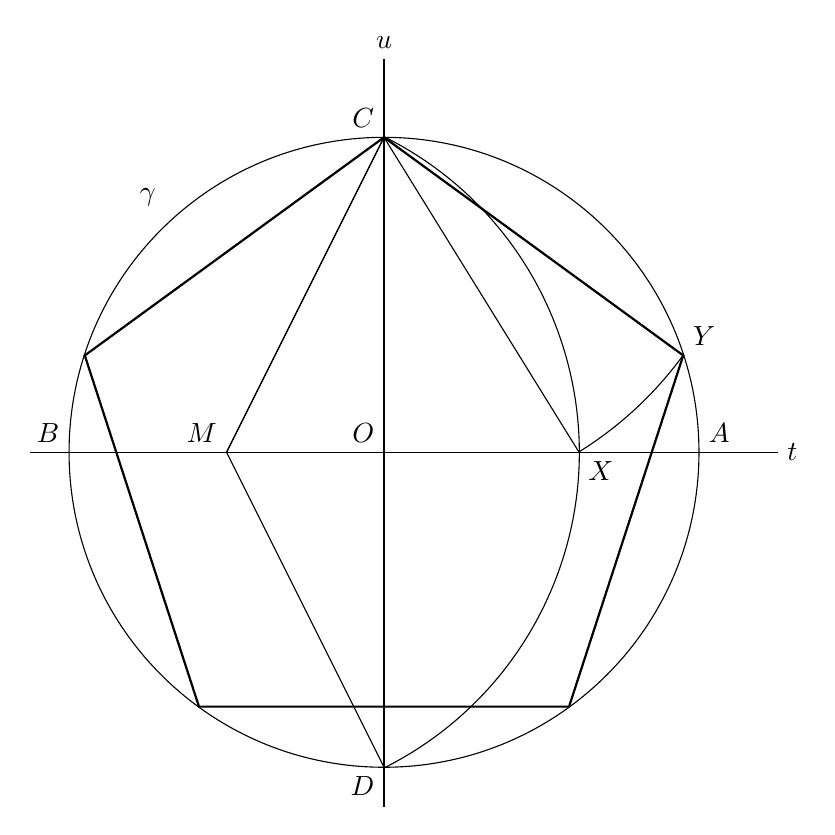
\begin{tikzpicture}
			\draw (0, 0) circle [radius=4];
			\coordinate[label=above left:$O$] (O) at (0,0);
			\coordinate[label=$\gamma$] (g) at (-3,3);
			\draw (-4.5, 0) -- (5, 0);
			\coordinate[label=right:$t$] (t) at (5,0);
			\coordinate[label=above right:$A$] (A) at (4,0);
			\coordinate[label=above left:$B$] (B) at (-4,0);
			\coordinate[label=above left:$M$] (M) at (-2,0);
			\draw (0,-4.5) -- (0,5);
			\coordinate[label=above:$u$] (u) at (0,5);
			\coordinate[label=above left:$C$] (C) at (0,4);
			\coordinate[label=below left:$D$] (D) at (0,-4);
			\draw (M) -- (C);
			\draw (M) -- (D);
			\draw (M) -- +(63.43:4.48) arc (63.43:-63.43:4.48);
			\coordinate[label=below right:$X$] (X) at (2.47,0);
			\draw (C) -- +(-58.23:4.7) arc (-58.23:-36:4.7);
			
			\coordinate[label=above right:$Y$] (Y) at (3.8,1.23);
			\coordinate (V) at (-3.8,1.23);
			\coordinate (W) at (-2.35,-3.23);
			\coordinate (Z) at (2.35,-3.23);
			
			\draw[thick] (Y) -- (C) -- (V) -- (W) -- (Z) -- cycle;		
		\end{tikzpicture}
	\end{figure} %
	
	% angle on a circunference.
	\begin{figure}
		\centering
		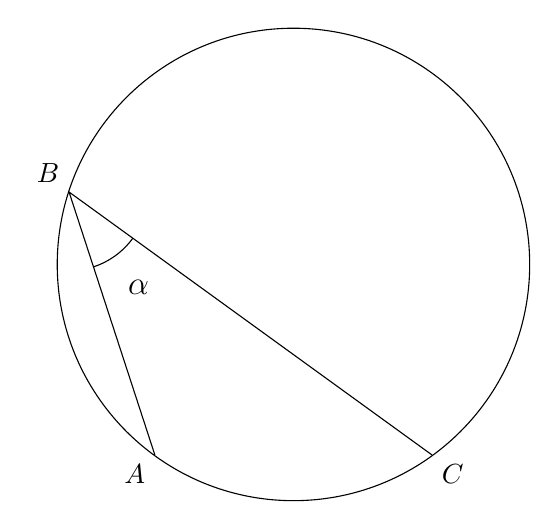
\begin{tikzpicture}
			\draw (0, 0) circle [radius=3]; 
			\coordinate[label=below left:$A$] (A) at (-1.76,-2.42);
			\coordinate[label=above left:$B$] (B) at (-2.85,0.92);
			\coordinate[label=below right:$C$] (C) at (1.76,-2.42);
			
			\draw (A) -- (B) -- (C);
			\draw pic["\large{$\alpha$}", draw=black, angle eccentricity=1.5, angle radius=1cm]{angle=A--B--C};		
		\end{tikzpicture}
	\end{figure} % 	
	
	% ADC 36° isosceles triangle inside regular pentagon.
	\begin{figure}
		\centering
		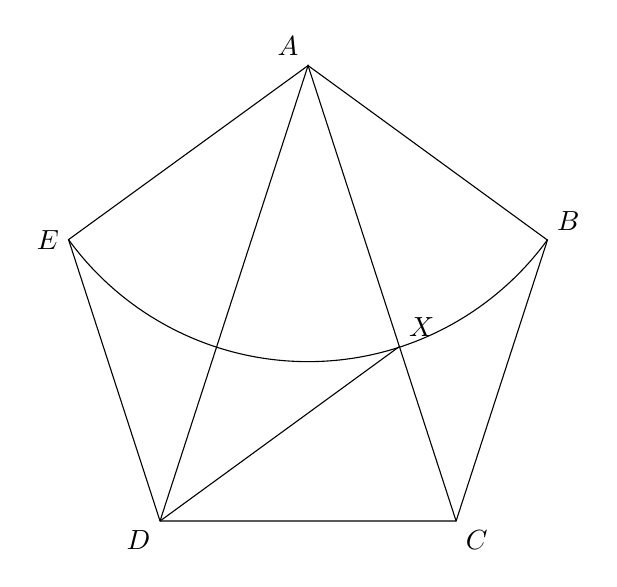
\begin{tikzpicture}[scale=0.8]			
			\coordinate[label=above left:$A$] (A) at (0,4);
			\coordinate[label=above right:$B$] (B) at (3.8,1.23);
			\coordinate[label=below right:$C$] (C) at (2.35,-3.23);
			\coordinate[label=below left:$D$] (D) at (-2.35,-3.23);
			\coordinate[label=left:$E$] (E) at (-3.8,1.23);
			
			\coordinate[label=above right:$X$] (X) at (1.45,-0.46);
			
			\draw (A) -- (B) -- (C) -- (D) -- (E);
			\draw (D) -- (A) -- (C);
			\draw (D) -- (X);		
			
			\draw (A) -- +(-144:4.7) arc (-144:-36:4.7);
		\end{tikzpicture}
	\end{figure} %	
	
	% angle bisector BD of an ABC 36° isosceles triangle.
	\begin{figure}
		\centering
		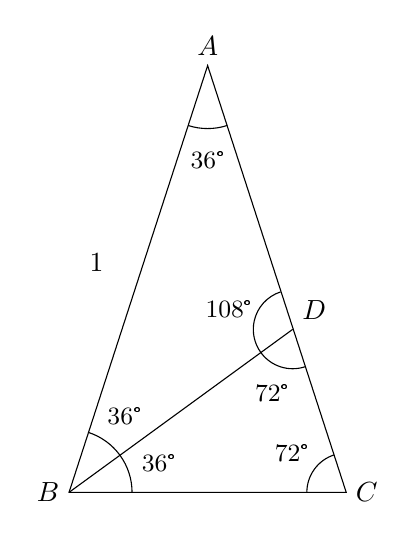
\begin{tikzpicture}
			\coordinate[label=above:$A$] (A) at (0,3);
			\coordinate[label=left:$B$] (B) at (-1.76,-2.42);
			\coordinate[label=right:$C$] (C) at (1.76,-2.42);
			\coordinate[label=above right:$D$] (D) at (1.08,-0.35);
			
			\coordinate[label=left:$1$] (O) at (-1.2,0.5);
			
			\draw (A) -- (B) -- (C) -- cycle;
			\draw (B) -- (D);
			
			\draw pic["\small{36°}", draw=black, angle eccentricity=1.5, angle radius=0.8cm]{angle=D--B--A};
			\draw pic["\small{36°}", draw=black, angle eccentricity=1.5, angle radius=0.8cm]{angle=C--B--D};	
			\draw pic["\small{36°}", draw=black, angle eccentricity=1.5, angle radius=0.8cm]{angle=B--A--C};	
			
			\draw pic["\small{72°}", draw=black, angle eccentricity=1.7, angle radius=0.5cm]{angle=B--D--C};
			\draw pic["\small{72°}", draw=black, angle eccentricity=1.7, angle radius=0.5cm]{angle=D--C--B};
			
			\draw pic["\small{108°}", draw=black, angle eccentricity=1.7, angle radius=0.5cm]{angle=A--D--B};
		\end{tikzpicture}
	\end{figure} %
	
	% projections of a point P inside an equilateral triangle.
	\begin{figure}
		\centering	
		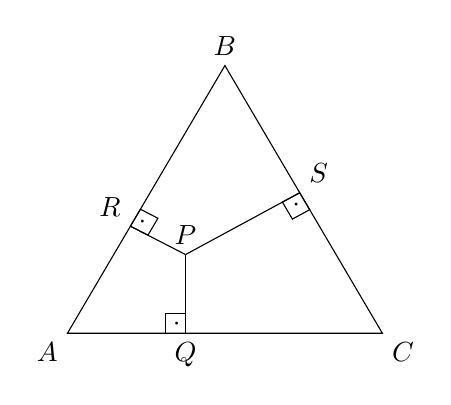
\begin{tikzpicture}
			\draw (0,0) -- (4,0) -- (2,3.4) -- cycle;
			
			\coordinate[label=below left:$A$] (A) at (0,0);
			\coordinate[label=above:$B$] (B) at (2,3.4);
			\coordinate[label=below right:$C$] (C) at (4,0);
			
			\coordinate[label=above: $P$] (P) at (1.5,1);
			\coordinate[label=below: $Q$] (Q) at (1.5,0);
			\coordinate[label=above left: $R$] (R) at (0.8, 1.36);
			\coordinate[label=above right: $S$] (S) at (2.95, 1.785);
			
			\draw (Q) -- (P);
			\tkzMarkRightAngle[size=0.25](P,Q,A);
			\tkzLabelAngle[dist=.16](P,Q,A){$\cdot$};
			
			\draw (R) -- (P);
			\tkzMarkRightAngle[size=0.25](P,R,B);
			\tkzLabelAngle[dist=.16](P,R,B){$\cdot$};
			
			\draw (S) -- (P);
			\tkzMarkRightAngle[size=0.25](P,S,C);
			\tkzLabelAngle[dist=.16](P,S,C){$\cdot$};
		\end{tikzpicture}
	\end{figure}	
		
	
	%%%%%%%%%%%%%%%%%%%%%%%%%%%%%%%%%%%%%%%%%%%%%%%%%%%%%%%%%%%%%%%%%%%%%%%%%%%%%%%%%%%%%%%
									      % graphs %
	%%%%%%%%%%%%%%%%%%%%%%%%%%%%%%%%%%%%%%%%%%%%%%%%%%%%%%%%%%%%%%%%%%%%%%%%%%%%%%%%%%%%%%%
	
	% series of transformations (T, h) on a function f.
	\begin{figure}[h!]\centering
		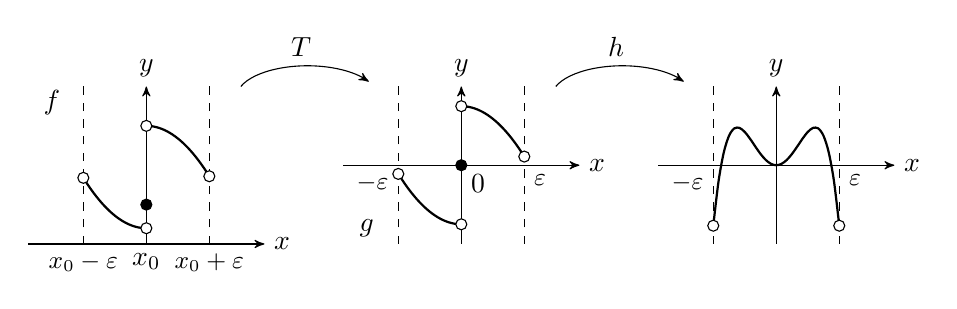
\begin{tikzpicture}[> = stealth']
			\draw [->] (-1.5, 0) -- (1.5,0) node [right] {$x$};
			\draw [->] (0,0) node [below] {$x_0$} -- (0,2) node [above] {$y$};
			
			\draw [dashed] (0.8, 0) node [below] {{\small$x_0+\varepsilon$}} --++ (0,2);
			\draw [dashed] (-0.8,0) node [below] {{\small$x_0-\varepsilon$}} --++ (0,2);
			
			\draw [thick, smooth, domain= 0:0.8] plot (\x, {1.5-\x*\x});
			\draw [thick, smooth, domain=-0.8:0] plot (\x, {0.2+\x*\x}); 
			
			\draw [fill=black] (0,0.5) circle (0.07cm);
			
			\draw [fill=white] (0.8 , 0.86) circle (0.07cm);
			\draw [fill=white] (-0.8, 0.84) circle (0.07cm);
			
			\draw [fill=white] (0, 0.2) circle (0.07cm);
			\draw [fill=white] (0, 1.5) circle (0.07cm);
			
			\node at (-1.2,1.8) {$f$};
			\node at (2.8, 0.2) {$g$};
			
			\draw [->] (1.2,2) arc (160:30:0.9 and 0.4) node [midway, above] {$T$};
			
			\begin{scope}[shift={(4,1)}]
				\draw [->] (-1.5, 0) -- (1.5, 0) node [right] {$x$};
				\draw [->] (0, -1) -- (0, 1) node [above] {$y$};
				
				\draw [dashed] (0.8, -1) -- (0.8, 1) node [midway, below 
				right]{{\small$\varepsilon$}};
				\draw [dashed] (-0.8,-1) -- (-0.8,1) node [midway, below left] {{\small$-\varepsilon$}};
				
				\draw [thick, smooth, domain= 0:0.8] plot (\x, {0.75-\x*\x});
				\draw [thick, smooth, domain=-0.8:0] plot (\x, {-0.75+\x*\x});
				
				\draw [fill=black] (0,0) circle (0.07cm) node [below right] {$0$};
				
				\draw [fill=white] (0.8 , 0.11) circle (0.07cm);
				\draw [fill=white] (-0.8, -0.11) circle (0.07cm);
				
				\draw [fill=white] (0, 0.75) circle (0.07cm);
				\draw [fill=white] (0,-0.75) circle (0.07cm);
				
				\draw [->] (1.2,1) arc (160:30:0.9 and 0.4) node [midway, above] {$h$};
			\end{scope}
			
			\begin{scope}[shift={(8,1)}]
				\draw [->] (-1.5, 0) -- (1.5, 0) node [right] {$x$};
				\draw [->] (0, -1) -- (0, 1) node [above] {$y$};
				
				\draw [dashed] (0.8, -1) -- (0.8, 1) node [midway, below 
				right]{{\small$\varepsilon$}};
				\draw [dashed] (-0.8,-1) -- (-0.8,1) node [midway, below left] {{\small$-\varepsilon$}};
				
				\draw [thick, domain=-0.8:0.8, smooth] plot (\x,
				 {-8*(\x*\x)*(\x-0.7)*(\x+0.7)});
				
				\draw [fill=white] (0.8 , -0.768) circle (0.07cm);
				\draw [fill=white] (-0.8, -0.768) circle (0.07cm);
			\end{scope}
		\end{tikzpicture}
	\end{figure} %
	
	% uniform convergence in action.
	\begin{figure}[h!]\centering
		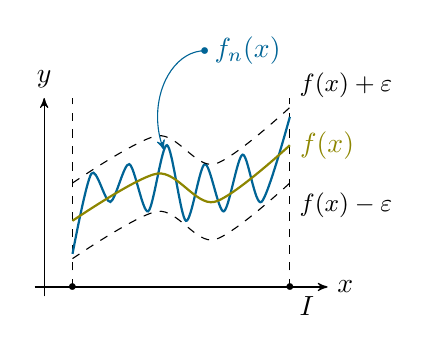
\begin{tikzpicture}[> = stealth', scale=1.2]
			\draw [->] (-0.1, 0) -- (3,0) node [right] {$x$};
			\draw [->] (0, -0.1) -- (0,2) node [above] {$y$};
			
			\draw [dashed] (0.3,0) node {{\tiny$\bullet$}} --++ (0,2); 
			\draw [dashed] (2.6,0) node {{\tiny$\bullet$}} node [below right] {$I$} --++ (0,2); 
			
			\draw [thick, smooth, marinho] plot coordinates
			{(0.3, 0.35) (0.5, 1.2) (0.7, 0.9) (0.9, 1.3) (1.1, 0.8) (1.3, 1.5) 
				(1.5, 0.7) (1.7, 1.3) (1.9, 0.8) (2.1, 1.4) (2.3, 0.9) (2.6, 1.8)};
			
			\draw [dashed, smooth] plot coordinates
			{(0.3,1.1) (1.2, 1.6) (1.8, 1.3) (2.6, 1.9)} node [above right] {{\small$f(x)+\varepsilon$}};
			
			\draw [thick, olive, smooth] plot coordinates
			{(0.3,0.7) (1.2, 1.2) (1.8, 0.9) (2.6, 1.5)} node [right] {$f(x)$};
			
			\draw [dashed, smooth] plot coordinates
			{(0.3,0.3) (1.2, 0.8) (1.8, 0.5) (2.6, 1.1)} node [below right] {{\small$f(x)-\varepsilon$}};
			
			\draw [->, marinho] (1.7, 2.5) node {{\tiny$\bullet$}} node [right] {$f_n(x)$}
			arc (90:210:0.5 and 0.7);
		\end{tikzpicture}
	\end{figure} %	
	
	% some probability production frontiers.
	\begin{figure}% portugal
		\centering
		\begin{subfigure}{0.4\textwidth}
			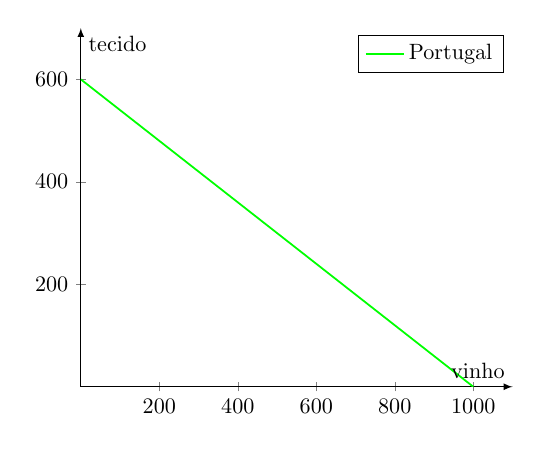
\begin{tikzpicture}[scale=0.8]
				\begin{axis}[
					axis x line = middle,    	 
					axis y line = middle,     
					axis line style = {-latex},
					xmin=0, xmax=11, ymin=0, ymax=7,
					xlabel = {vinho},		
					xtick = {2,4,6,8,10},
					xticklabels = {$200$,$400$,$600$,$800$,$1000$},
					ylabel = {tecido},
					ytick = {2,4,6},
					yticklabels = {$200$,$400$,$600$}
					]
					\addplot +[mark=none, green, thick] coordinates {(0,6) (10,0)};
					\legend{Portugal}
				\end{axis}
			\end{tikzpicture}
		\end{subfigure}
		\hfill
		\begin{subfigure}{0.4\textwidth}% inglaterra
			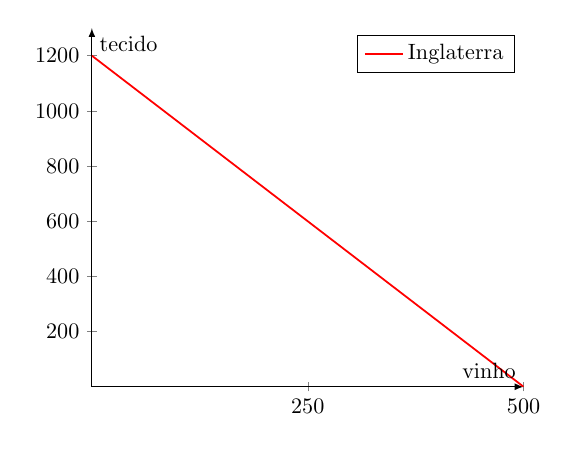
\begin{tikzpicture}[scale=0.8]
				\begin{axis}[
					axis x line = middle,    	 
					axis y line = middle,     
					axis line style = {-latex},
					xmin=0, xmax=5, ymin=0, ymax=13,
					xlabel = {vinho},		
					xtick = {2.5,5},
					xticklabels = {$250$,$500$},
					ylabel = {tecido},
					ytick = {2,4,6,8,10,12},
					yticklabels = {$200$,$400$,$600$,$800$,$1000$,$1200$}
					]
					\addplot +[mark=none, red, thick] coordinates {(0,12) (5,0)};
					\legend{Inglaterra}
				\end{axis}
			\end{tikzpicture}
		\end{subfigure}
	\end{figure} %	
	\begin{figure} % second green line
		\centering
		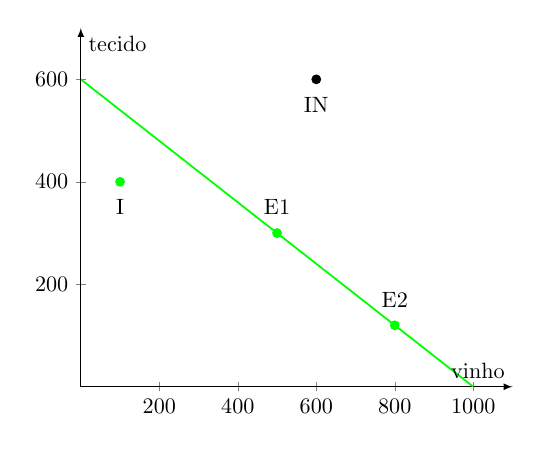
\begin{tikzpicture}[scale=0.8]
			\begin{axis}[
				axis x line = middle,    	 
				axis y line = middle,     
				axis line style = {-latex},
				xmin=0, xmax=11, ymin=0, ymax=7,
				xlabel = {vinho},		
				xtick = {2,4,6,8,10},
				xticklabels = {$200$,$400$,$600$,$800$,$1000$},
				ylabel = {tecido},
				ytick = {2,4,6},
				yticklabels = {$200$,$400$,$600$}
				]
				\addplot +[mark=none, green, thick] coordinates {(0,6) (10,0)};
				\addplot[soldot] coordinates{(1,4)};
				\node at (1,3.5) {I};
				
				\addplot[soldot] coordinates{(5,3)};
				\node at (5,3.5) {E$1$};
				
				\addplot[soldot] coordinates{(8,1.2)};
				\node at (8,1.7) {E$2$};
				
				\addplot[holdot] coordinates{(6,6)};
				\node at (6,5.5) {IN};
			\end{axis}
		\end{tikzpicture}
	\end{figure} %
	
	% graphs of the hyperbolas xy = k^2.
	\begin{figure}
		\centering
		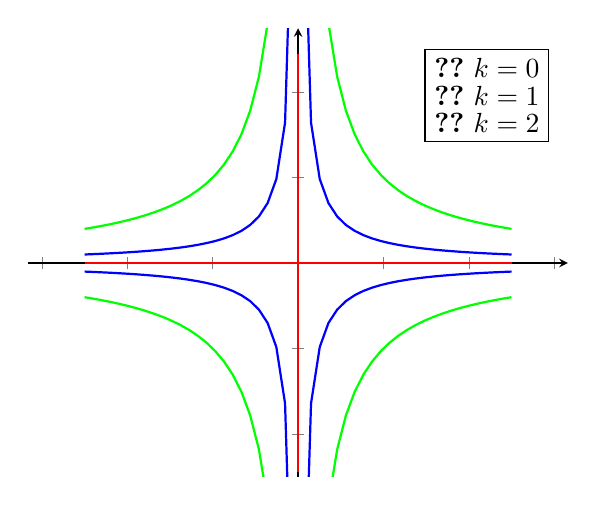
\begin{tikzpicture}
			\begin{axis}[
				axis lines = middle,
				xmin=-5, xmax=5, ymin=-5, ymax=5.5,
				axis equal,
				xlabel = {},
				xticklabels = {},
				ylabel = {},
				yticklabels = {}
				]
				\addplot[domain=-5:5, red, thick] {0};
				\addplot +[mark=none] coordinates {(0,-4.9) (0,4.9)};
				\label{0}
				
				\addplot[domain=0.1:5, blue, thick] {1/x};
				\addplot[domain=-5:-0.1, blue, thick] {1/x};
				\addplot[domain=0.1:5, blue, thick] {-1/x};
				\addplot[domain=-5:-0.1, blue, thick] {-1/x};
				\label{1}
				
				\addplot[domain=0.1:5, green, thick] {4/x};
				\addplot[domain=-5:-0.1, green, thick] {4/x};
				\addplot[domain=0.1:5, green, thick] {-4/x};
				\addplot[domain=-5:-0.1, green, thick] {-4/x};
				\label{2}
				
				\node [draw,fill=white] at (rel axis cs: 0.85,0.85) {\shortstack[l]{
						\ref{0} $k=0$ \\
						\ref{1} $k=1$ \\
						\ref{2} $k=2$}};
			\end{axis}
		\end{tikzpicture}
	\end{figure} %	
	
	% some more graphs; x^2, 8x^2, xy=1, xy=27.
	\begin{figure}[h!]\centering
		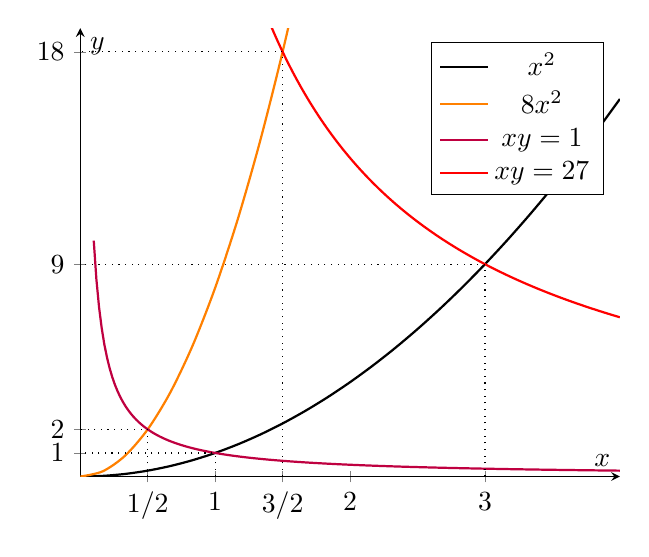
\begin{tikzpicture}
			\begin{axis}[
				legend pos = north east, 
				axis lines = middle,
				xmin = 0, xmax = 4, xlabel = {$x$},
				ymin = 0, ymax = 19, ylabel = {$y$},
				xtick = {0.5, 1, 1.5, 2, 3},
				xticklabels={1/2,1,3/2,2,3},
				ytick = {1,2,9,18}, yticklabels = {1,2,9,18}]	     
				
				\addplot[thick, smooth, domain=0:4] {x*x};
				\addplot[thick, smooth, domain=0:4, orange] {8*x*x};
				
				\addplot[thick, samples=200, blue, domain=0.1:4,
				purple] {1/x};
				\addplot[thick, samples=200, blue, domain=0.1:4,
				red]{27/x};
				
				\draw[dotted] (1,0)--(1,1)--(0,1);
				\draw[dotted] (0.5,0)--(0.5,2)--(0,2);
				\draw[dotted] (1.5,0)--(1.5,18)--(0,18);
				\draw[dotted] (3,0)--(3,9)--(0,9);
				
				\legend{$x^2$, $8x^2$, $xy=1$, $xy=27$};
			\end{axis}
		\end{tikzpicture}
	\end{figure} %


	%%%%%%%%%%%%%%%%%%%%%%%%%%%%%%%%%%%%%%%%%%%%%%%%%%%%%%%%%%%%%%%%%%%%%%%%%%%%%%%%%%%%%%%
	                              % logical circuits %
	%%%%%%%%%%%%%%%%%%%%%%%%%%%%%%%%%%%%%%%%%%%%%%%%%%%%%%%%%%%%%%%%%%%%%%%%%%%%%%%%%%%%%%%
	
	% flip-flop JK.
	\begin{figure}[h!]\centering
		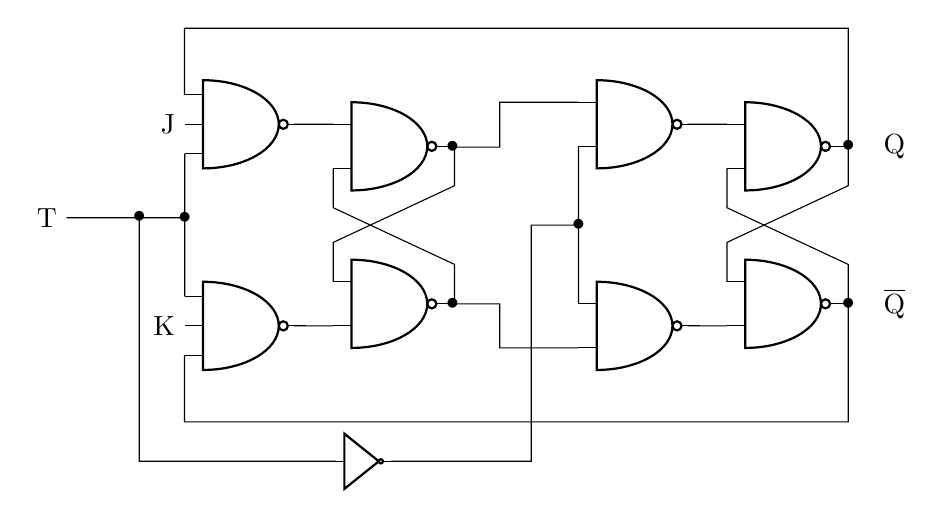
\begin{tikzpicture}
			\draw
			(0,2) node[nand port] (NAND1) {}
			(0,0) node[nand port] (NAND2) {}
			
			(NAND1.in 1) --++ (-0.5,0) node [nand port, number inputs=3] (NANDT1) {}
			(NAND2.in 2) --++ (-0.5,0) node [nand port, number inputs=3] (NANDT2) {}
			
			(NANDT1.in 2) node[anchor=east] {J} 
			(NANDT2.in 2) node[anchor=east] {K} 
			
			(NANDT1.in 3) --++ (0,-1)
			(NANDT2.in 1) --++ (0,+1) node {{\small$\bullet$}}
			--++ (-1.5,0) node [anchor=east] {T}
			
			(NAND1.out) -- ++(0,-0.5) -- ($(NAND2.in 1) +(0,0.5)$) -- (NAND2.in 1)
			(NAND2.out) -- ++(0,+0.5) -- ($(NAND1.in 2) +(0,-0.5)$)--(NAND1.in 2);
			
			\begin{scope}[shift={(5,0)}]
				\draw
				(-6,-2) node [not port, scale=0.5] (NOT) {}
				
				(0,2) node[nand port] (NAND1) {}
				(1,2) node[anchor=east] {Q}
				(1,0) node[anchor=east] {$\overline{\text{Q}}$}
				(0,0) node[nand port] (NAND2) {}
				
				(NAND1.in 1) --++ (-0.5,0) node [nand port] (NANDT1) {}
				(NAND2.in 2) --++ (-0.5,0) node [nand port] (NANDT2) {}
				
				(NANDT1.in 1) --++ (-1,0) --++ (0,-0.57) --++ (-0.6,0) node {{\small$\bullet$}}
				(NANDT2.in 2) --++ (-1,0) --++ (0,+0.56) --++ (-0.6,0) node {{\small$\bullet$}}
				
				(NANDT1.in 2) --++ (0,-1)
				(NANDT2.in 1) --++ (0,+1) node {{\small$\bullet$}}
				--++ (-0.6,0) --++ (0,-3) -- (NOT.out) 
				
				(NAND1.out) -- ++(0,-0.5) -- ($(NAND2.in 1) +(0,0.5)$) -- (NAND2.in 1)
				(NAND2.out) -- ++(0,+0.5) -- ($(NAND1.in 2) +(0,-0.5)$)--(NAND1.in 2)
				
				(NAND1.out) node {{\small$\bullet$}} --++ (0,1.5) --++ (-8.43,0) --++ (0,-0.85)
				(NAND2.out) node {{\small$\bullet$}} --++ (0,-1.5) --++ (-8.43,0) --++ (0,+0.85)
				
				(NOT.in) --++ (-2.5,0) --++ (0,3.1) node {{\small$\bullet$}}
				;
			\end{scope}
		\end{tikzpicture}
	\end{figure} %
	
	% master-slave flip-flop RS.
	\begin{figure}[h!]\centering
		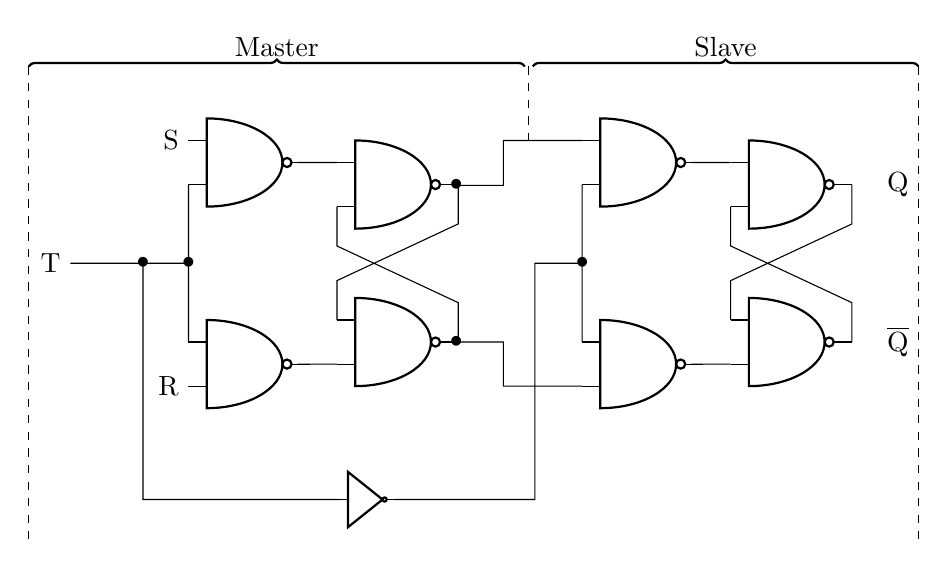
\begin{tikzpicture}
			\draw [decorate, thick, decoration = {brace}] 
			(-5.3,3.5) --  (1,3.5) node [midway, above] {Master};
			
			\draw [decorate, thick, decoration = {brace}]
			(1.1, 3.5) -- (6, 3.5) node [midway, above] {Slave};
			
			\draw [dashed] (-5.3, 3.5) --++ (0,-6);
			\draw [dashed] (1.05, 3.5) --++ (0,-1);
			\draw [dashed] (6, 3.5) --++ (0, -6);
			
			\draw
			(0,2) node[nand port] (NAND1) {}
			(0,0) node[nand port] (NAND2) {}
			
			(NAND1.in 1) --++ (-0.5,0) node [nand port] (NANDT1) {}
			(NAND2.in 2) --++ (-0.5,0) node [nand port] (NANDT2) {}
			
			(NANDT1.in 1) node[anchor=east] {S} 
			(NANDT2.in 2) node[anchor=east] {R} 
			
			(NANDT1.in 2) --++ (0,-1)
			(NANDT2.in 1) --++ (0,+1) node {{\small$\bullet$}}
			--++ (-1.5,0) node [anchor=east] {T}
			
			(NAND1.out) -- ++(0,-0.5) -- ($(NAND2.in 1) +(0,0.5)$) -- (NAND2.in 1)
			(NAND2.out) -- ++(0,+0.5) -- ($(NAND1.in 2) +(0,-0.5)$)--(NAND1.in 2);
			
			\begin{scope}[shift={(5,0)}]
				\draw
				(-6,-2) node [not port, scale=0.5] (NOT) {}
				
				(0,2) node[nand port] (NAND1) {}
				(1,2) node[anchor=east] {Q}
				(1,0) node[anchor=east] {$\overline{\text{Q}}$}
				(0,0) node[nand port] (NAND2) {}
				
				(NAND1.in 1) --++ (-0.5,0) node [nand port] (NANDT1) {}
				(NAND2.in 2) --++ (-0.5,0) node [nand port] (NANDT2) {}
				
				(NANDT1.in 1) --++ (-1,0) --++ (0,-0.57) --++ (-0.6,0) node {{\small$\bullet$}}
				(NANDT2.in 2) --++ (-1,0) --++ (0,+0.56) --++ (-0.6,0) node {{\small$\bullet$}}
				
				(NANDT1.in 2) --++ (0,-1)
				(NANDT2.in 1) --++ (0,+1) node {{\small$\bullet$}}
				--++ (-0.6,0) --++ (0,-3) -- (NOT.out) 
				
				(NAND1.out) -- ++(0,-0.5) -- ($(NAND2.in 1) +(0,0.5)$) -- (NAND2.in 1)
				(NAND2.out) -- ++(0,+0.5) -- ($(NAND1.in 2) +(0,-0.5)$)--(NAND1.in 2)
				
				(NOT.in) --++ (-2.5,0) --++ (0,3) node {{\small$\bullet$}}
				;
			\end{scope}
		\end{tikzpicture}
	\end{figure} %
	
	% triggered latch RS
	\begin{figure}[h!]
		\centering
			\begin{circuitikz}
				\draw [decorate, thick, decoration = {brace}] 
				(-4.3,3.5) --  (-1.7,3.5) node [midway, above] {Trigger};
				\draw [dashed] (-1.7,3.5) --++ (0,-4.5);
				\draw [dashed] (-4.3,3.5) --++ (0,-4.5);
				
				\draw
				(0,2) node[nand port] (NAND1) {}
				(1,2) node[anchor=east] {Q}
				(1,0) node[anchor=east] {$\overline{\text{Q}}$}
				(0,0) node[nand port] (NAND2) {}
				
				(NAND1.in 1) --++ (-0.5,0) node [nand port] (NANDT1) {}
				(NAND2.in 2) --++ (-0.5,0) node [nand port] (NANDT2) {}
				
				(NANDT1.in 1) node[anchor=east] {S} 
				(NANDT2.in 2) node[anchor=east] {R} 
				
				(NANDT1.in 2) --++ (0,-1)
				(NANDT2.in 1) --++ (0,+1) node {{\small$\bullet$}}--++ (-0.5,0) node [anchor=east] {T}
				
				(NAND1.out) -- ++(0,-0.5) -- ($(NAND2.in 1) +(0,0.5)$) -- (NAND2.in 1)
				(NAND2.out) -- ++(0,+0.5) -- ($(NAND1.in 2) +(0,-0.5)$)--(NAND1.in 2);
			\end{circuitikz}
	\end{figure}
	
	% flip-flop D
	\begin{figure}[h!]\centering
		\begin{circuitikz}
			\draw
			(0,0) node [nand port] (NAND1) {} ++
			(0,2) node [nand port] (NAND2) {} 
			
			(-2.5, 3) node [anchor=east] {Clk} ++ 
			(5,0) node [nand port, number inputs = 3] (NAND3) {} ++
			(0,2) node [nand port] (NAND4) {}
			
			(NAND3.out) ++ (2,-0.28) node [nand port] (NAND5) {} 
			++ (0,-2) node [nand port] (NAND6) {} ;
			\draw 
			(NAND2.out) -- ++(0,-0.5) -- ($(NAND1.in 1) +(0,0.5)$) -- (NAND1.in 1)
			(NAND1.out) -- ++(0,+0.5) -- ($(NAND2.in 2) +(0,-0.5)$)-- (NAND2.in 2)
			
			(NAND5.out) -- ++(0,-0.5) -- ($(NAND6.in 1) +(0,0.5)$) -- (NAND6.in 1)
			(NAND6.out) -- ++(0,+0.5) -- ($(NAND5.in 2) +(0,-0.5)$)-- (NAND5.in 2)
			
			(NAND4.out) -- ++(0,-0.5) -- ($(NAND3.in 1) +(0,0.5)$) -- (NAND3.in 1)
			(NAND3.out) -- ++(0,+0.5) -- ($(NAND4.in 2) +(0,-0.5)$)-- (NAND4.in 2)
			
			(NAND3.in 2) --++ (-3.5,0)
			(NAND3.in 3) --++ (0,-2.65) -- (NAND1.out) node {{\small$\bullet$}}
			(NAND3.out) -- (NAND5.in 1)
			
			(NAND6.in 2) --++ (-2.15,0) node {{\small$\bullet$}}
			(NAND1.in 2) --++ (-0.5,0) --++ (0,3.27) node {{\small$\bullet$}}
			(NAND2.in 1) --++ (0,1.1) -- (NAND3.in 1) node {{\small$\bullet$}}
			(NAND4.in 1) --++ (-3.5,0) node [anchor=east] {D}
			
			(NAND5.out) node [anchor=west] {$\overline{\text{Q}}$}
			(NAND6.out) node [anchor=west] {Q};
			
			\begin{scope}[shift={(6,3.5)}]
				\draw 
				(-0.5,4/3) --++ (0.5,0) node [right] {D}
				(-0.5,2/3) --++ (0.5,0) node [right] {Clk}
				(1.5, 4/3) node [left] {Q} --++ (0.5,0)
				(1.5, 2/3) node [left] {$\overline{\text{Q}}$} --++ (0.5,0)
				(0,0) rectangle (1.5,2)
				(0, 2/3+0.1) -- (0.14,2/3) -- (0,2/3-0.1)
				;
			\end{scope}
		\end{circuitikz}
	\end{figure} %
	
	% Latch D
	\begin{figure}[h!]\centering
		\begin{circuitikz}
			\draw
			(0,2) node[nand port] (NAND1) {}
			(1,2) node[anchor=east] {Q}
			(1,0) node[anchor=east] {$\overline{\text{Q}}$}
			(0,0) node[nand port] (NAND2) {}
			
			(NAND1.in 1) --++ (-0.5,0) node [nand port] (NANDT1) {}
			(NAND2.in 2) --++ (-0.5,0) node [nand port] (NANDT2) {}
			
			(NANDT1.in 1) --++ (-2,0) node [anchor=east] {D}
			(NANDT2.in 2) ++ (-0.7,0) node[not port, scale=0.5] (NOT) {}
			
			(NOT.out) -- (NANDT2.in 2)
			(NOT.in) --++ (-0.2,0) --++ (0,3.1) node {{\small$\bullet$}}
			
			(NANDT1.in 2) --++ (0,-1)
			(NANDT2.in 1) --++ (0,+1) node {{\small$\bullet$}}--++ (-0.3,0) node [anchor=east] {Clk}
			
			(NAND1.out) -- ++(0,-0.5) -- ($(NAND2.in 1) +(0,0.5)$) -- (NAND2.in 1)
			(NAND2.out) -- ++(0,+0.5) -- ($(NAND1.in 2) +(0,-0.5)$)--(NAND1.in 2);
			
			\node at (1.6,1) {{\Huge$\equiv$}};
			
			\begin{scope}[shift={(3,0)}]
				\draw (-0.5,4/3) --++ (0.5,0) node [right] {D}
				(-0.5,2/3) --++ (0.5,0) node [right] {Clk}
				(0,2/3+0.1) --++ (0.1,-0.1) --++ (-0.1,-0.1)
				(1.5, 4/3) node [left] {Q} --++ (0.5,0)
				(1.5, 2/3) node [left] {$\overline{\text{Q}}$} --++ (0.5,0)
				(0,0) rectangle (1.5,2);
			\end{scope}
		\end{circuitikz}
	\end{figure} %
	
	% sybchronous 4-bit counter implemented with flip-flops JK.
	\begin{figure}[h!]\centering
		\begin{tikzpicture}[thick]
			%% FF JK
			\draw (0,0) rectangle ++(1.5, 2) 
			(3,0) rectangle ++(1.5, 2)
			(6,0) rectangle ++(1.5, 2)
			(9,0) rectangle ++(1.5, 2)
			%
			(0.3, 1.6) node {$D_0$} ++ 
			(3, 0) node {$D_1$} ++
			(3, 0) node {$D_2$} ++
			(3, 0) node {$D_3$}
			%
			(1.15, 1.6) node {$Q_0$} ++
			(3, 0) node {$Q_1$} ++
			(3, 0) node {$Q_2$} ++
			(3, 0) node {$Q_3$}
			%
			(1.15, 0.4) node {$\overline{Q}_0$} ++
			(3, 0) node {$\overline{Q}_1$} ++
			(3, 0) node {$\overline{Q}_2$} ++
			(3, 0) node {$\overline{Q}_3$}
			%
			(0,0.55) --++ (0.1,-0.2) --++ (-0.1,-0.2) -- cycle ++
			(3,0) --++ (0.1,-0.2) --++ (-0.1,-0.2) -- cycle ++
			(3,0) --++ (0.1,-0.2) --++ (-0.1,-0.2) -- cycle ++
			(3,0) --++ (0.1,-0.2) --++ (-0.1,-0.2) -- cycle 
			% 
			(0.45, 0.35) node {Clk} ++ 
			(3, 0) node {Clk}++ 
			(3, 0) node {Clk}++ 
			(3, 0) node {Clk}
			%
			(1.5, 1.6) --++ (1.5, 0) ++ 
			(1.5, 0) --++ (1.5, 0) ++
			(1.5, 0) --++ (1.5, 0) ++
			(1.5, 0) --++ (0.75, 0) --++ (0,1) --++ (-11.75,0) --++ 
			(0,-1) --++ (0.5, 0)
			%
			(2.25, 1.6) node {$\bullet$} --++ (0,-0.4) node [below] {$Q_0$}
			(5.25, 1.6) node {$\bullet$} --++ (0,-0.4) node [below] {$Q_1$}
			(8.25, 1.6) node {$\bullet$} --++ (0,-0.4) node [below] {$Q_2$}
			(11.25, 1.6) node {$\bullet$} --++ (0,-0.4) node [below] {$Q_3$}
			%
			(0, 0.35) --++ (-0.75, 0) node {$\bullet$} --++ (0,-1)
			--++ (9,0)
			(3, 0.35) --++ (-0.75, 0) --++ (0,-1) node {$\bullet$}
			(6, 0.35) --++ (-0.75, 0) --++ (0,-1) node {$\bullet$}
			(9, 0.35) --++ (-0.75, 0) --++ (0,-1)
			;
			
			\draw 
			(0,0.35) ++ (-1.5,0) node [left]
			{\begin{tikzpicture}[thick]
					\draw (0,0) --++ (0.1, 0) --++ (0, 0.4) --++ 
					(0.3, 0) --++ (0, -0.4) --++ (0.1, 0);
					\draw (-0.1, -0.1) rectangle (0.6, 0.5);
				\end{tikzpicture}
			}
			(0,0.35) --++ (-1.65, 0);
		\end{tikzpicture}
	\end{figure} 
	
	% asynchronous 4-bit counter implemented with flip-flops JK.
	\begin{figure}[h!]\centering
		\begin{tikzpicture}[thick]
			%% FF JK
			\draw (0,0) rectangle ++(1.5, 2) 
			(3,0) rectangle ++(1.5, 2)
			(6,0) rectangle ++(1.5, 2)
			(9,0) rectangle ++(1.5, 2)
			%
			(0.3, 1.6) node {$J_0$} ++ 
			(3, 0) node {$J_1$} ++
			(3, 0) node {$J_2$} ++
			(3, 0) node {$J_3$}
			%
			(0.35, 0.35) node {$K_0$} ++
			(3, 0) node {$K_1$} ++
			(3, 0) node {$K_2$} ++
			(3, 0) node {$K_3$}
			%
			(1.15, 1.6) node {$Q_0$} ++
			(3, 0) node {$Q_1$} ++
			(3, 0) node {$Q_2$} ++
			(3, 0) node {$Q_3$}
			%
			(1.15, 0.4) node {$\overline{Q}_0$} ++
			(3, 0) node {$\overline{Q}_1$} ++
			(3, 0) node {$\overline{Q}_2$} ++
			(3, 0) node {$\overline{Q}_3$}
			%
			(0,1.2) --++ (0.1,-0.2) --++ (-0.1,-0.2) -- cycle ++
			(3,0) --++ (0.1,-0.2) --++ (-0.1,-0.2) -- cycle ++
			(3,0) --++ (0.1,-0.2) --++ (-0.1,-0.2) -- cycle ++
			(3,0) --++ (0.1,-0.2) --++ (-0.1,-0.2) -- cycle 
			% 
			(0.45, 1) node {Clk} ++ 
			(3, 0) node {Clk}++ 
			(3, 0) node {Clk}++ 
			(3, 0) node {Clk}
			%
			(0, 0.35) --++ (-0.6,0) --++ (0,2) node{$\bullet$} 
			--++ (0,-0.75) node {$\bullet$}
			--++ (0.6, 0) -- cycle
			++ (3,0)
			--++ (-0.6,0) --++ (0,2) node{$\bullet$} 
			--++ (0,-0.75) node {$\bullet$}
			--++ (0.6, 0) -- cycle
			++ (3,0)
			--++ (-0.6,0) --++ (0,2) node{$\bullet$} 
			--++ (0,-0.75) node {$\bullet$}
			--++ (0.6, 0) -- cycle
			++ (3,0)
			--++ (-0.6,0) --++ (0,2) node{$\bullet$} 
			--++ (0,-0.75) node {$\bullet$}
			--++ (0.6, 0) -- cycle
			%
			(8.4, 2.35) --++ (-9,0) --++ (0, 0.5) node [above] {Vcc}
			%
			(1.5, 1.6) --++ (0.6, 0) --++ (0, -0.6) node {$\bullet$} 
			--++ (0.9,0) ++ (-0.9, 0) --++ (0, -1.2) node [below] {$Q_0$}
			++ (-0.6, 1.8) ++
			%
			(3, 0) --++ (0.6, 0) --++ (0, -0.6) node {$\bullet$} 
			--++ (0.9,0) ++ (-0.9, 0) --++ (0, -1.2) node [below] {$Q_1$}
			++ (-0.6, 1.8) ++
			%
			(3, 0) --++ (0.6, 0) --++ (0, -0.6) node {$\bullet$} 
			--++ (0.9,0) ++ (-0.9, 0) --++ (0, -1.2) node [below] {$Q_2$}
			++ (-0.6, 1.8) ++
			%
			(3, 0) --++ (0.6, 0) --++  (0, -1.8) node [below] {$Q_3$}
			;
			
			\draw (0,1) ++ (-1,0) node [left]
			{\begin{tikzpicture}[thick]
					\draw (0,0) --++ (0.1, 0) --++ (0, 0.4) --++ 
					(0.3, 0) --++ (0, -0.4) --++ (0.1, 0);
					\draw (-0.1, -0.1) rectangle (0.6, 0.5);
				\end{tikzpicture}
			}
			(0,1) --++ (-1.15, 0);
			
			\draw [fill=white] (-0.1, 1) circle (0.1) ++
			(3,0) circle (0.1)++
			(3,0) circle (0.1)++
			(3,0) circle (0.1);
		\end{tikzpicture}
	\end{figure} %
	
	% NOR and NAND logical gates
	\begin{figure}[h!]
		\centering
		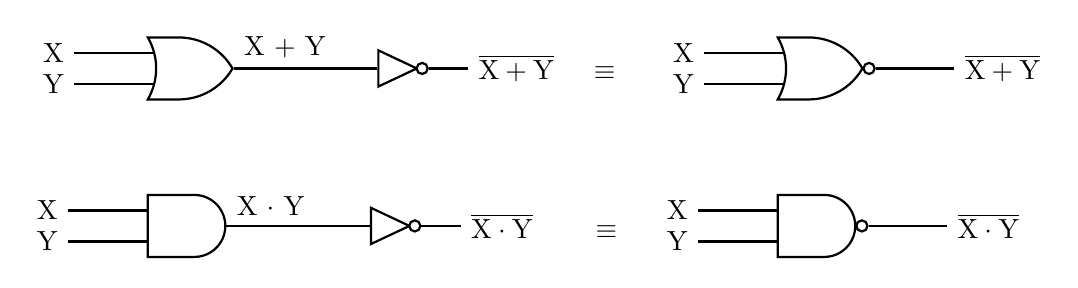
\begin{tikzpicture}[
			thick,
			GateCfg/.style={
				logic gate inputs={normal, normal, normal},
				draw, scale=1
			}
			]
			
			\path
			(0,0) node [or gate US, GateCfg] (OR) {} 
			(OR.input 1) ++ (-1, 0)  
			(OR.input 3) ++ (-1, 0) 
			(OR.output)  ++ ( 2, 0) node [not gate US, draw] (NOT) {};
			
			\draw 
			(OR.input 1) -- ++ (-1,0) node [at end, left] {X}
			(OR.input 3) -- ++ (-1,0) node [at end, left] {Y}
			(OR.output) -- (NOT.input) node[at start, above right] {X $+$ Y}
			(NOT.output) -- ++ (0.5,0) node [at end, right] 
			{$\overline{\text{X}+\text{Y}}\quad\,\equiv$};
			
			\begin{scope}[shift={(8,0)}]
				
				\path 
				(0,0) node [nor gate US, GateCfg] (NOR) {}
				(NOR.input 1) ++ (-1, 0)  
				(NOR.input 3) ++ (-1, 0);
				
				\draw
				(NOR.input 1) -- ++ (-1, 0) node [at end, left] {X}
				(NOR.input 3) -- ++ (-1, 0) node [at end, left] {Y}
				(NOR.output) -- ++ (1,0) node [at end, right] {$\overline{\text{X}+\text{Y}}$}; 
			\end{scope}
			
			\begin{scope}[shift={(0,-2)}]
				\path
				(0,0) node [and gate US, GateCfg] (AND) {} 
				(AND.input 1) ++ (-1, 0)  
				(AND.input 3) ++ (-1, 0) 
				(AND.output)  ++ ( 2, 0) node [not gate US, draw] (NOT) {};
				
				\draw 
				(AND.input 1) -- ++ (-1,0) node [at end, left] {X}
				(AND.input 3) -- ++ (-1,0) node [at end, left] {Y}
				(AND.output) -- (NOT.input) node[at start, above right] {X $\cdot$ Y}
				(NOT.output) -- ++ (0.5,0) node [at end, right] 
				{$\overline{\text{X}\cdot\text{Y}}\qquad\equiv$};
				
				\begin{scope}[shift={(8,0)}]
					
					\path 
					(0,0) node [nand gate US, GateCfg] (NAND) {}
					(NAND.input 1) ++ (-1, 0)  
					(NAND.input 3) ++ (-1, 0);
					
					\draw
					(NAND.input 1) -- ++ (-1, 0) node [at end, left] {X}
					(NAND.input 3) -- ++ (-1, 0) node [at end, left] {Y}
					(NAND.output) -- ++ (1,0) node [at end, right] {$\overline{\text{X}\cdot\text{Y}}$}; 
				\end{scope}
			\end{scope}
		\end{tikzpicture}
	\end{figure} %	
	
	% XOR logic gate as an association of NAND gates
	\begin{figure}[h!]\centering
		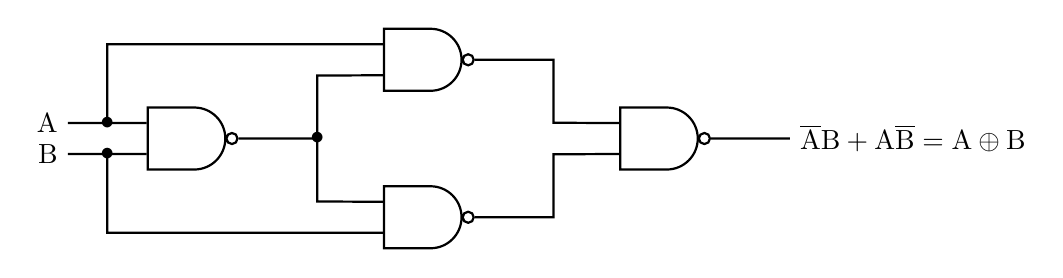
\begin{tikzpicture}[
			thick,
			GateCfg/.style={
				logic gate inputs = {normal, normal, normal},
				draw
			}
			]
			
			\path 
			(0,0) node [nand gate US, GateCfg] (NAND1) {}
			++ (3,1) node [nand gate US, GateCfg] (NAND2) {}
			++ (0,-2) node [nand gate US, GateCfg] (NAND3) {}
			++ (3,1) node [nand gate US, GateCfg] (NAND4) {};
			
			\draw
			(NAND1.input 1) --++ (-1,0) node [at end, left] {A}
			(NAND1.input 3) --++ (-1,0) node [at end, left] {B}
			
			(NAND1.output) --++ (1,0) node {$\bullet$} --++ (0, -0.8) -- (NAND3.input 1)
			(NAND1.output) --++ (1,0) --++ (0, 0.8) -- (NAND2.input 3)
			
			(NAND2.input 1) --++ (-3.5,0) --++ (0,-1) node {$\bullet$}
			(NAND3.input 3) --++ (-3.5,0) --++ (0, 1) node {$\bullet$}
			
			(NAND2.output) --++ (1,0) --++ (0,-0.8) -- (NAND4.input 1)
			(NAND3.output) --++ (1,0) --++ (0, 0.8) -- (NAND4.input 3)
			
			(NAND4.output) --++ (1,0) node [at end, right] 
			{$\overline{\text{A}}\text{B}+\text{A}\overline{\text{B}} =
				\text{A}\oplus\text{B}$};
		\end{tikzpicture}
	\end{figure} %


	%%%%%%%%%%%%%%%%%%%%%%%%%%%%%%%%%%%%%%%%%%%%%%%%%%%%%%%%%%%%%%%%%%%%%%%%%%%%%%%%%%%%%%%
						        % diagrams on the complex plane %
	%%%%%%%%%%%%%%%%%%%%%%%%%%%%%%%%%%%%%%%%%%%%%%%%%%%%%%%%%%%%%%%%%%%%%%%%%%%%%%%%%%%%%%%
	
	% Möbius transformation S, its image on the upper semi-plane, and inverse. 
	\begin{figure}[h!]\centering
		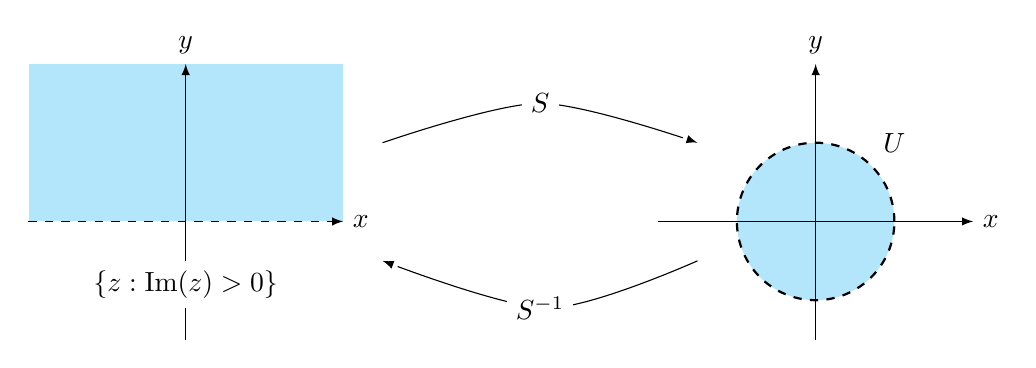
\begin{tikzpicture}
			%% Domínio
			\draw [thin, color=white, fill=cyan!30] (-2,2)--(-2,0)--(2,0)--(2,2);
			
			%% Eixos  da esquerda
			\draw [-latex, dashed] (-2,0)--(2,0) node [at end, right] {$x$};
			\draw [-latex] (0,-1.5)--(0,2)  node [at end, above] {$y$}; 
			
			%% Aplicação
			\draw[-latex] plot [smooth] coordinates {(2.5,1) (4.5,1.5) (6.5,1)}
			node [at={(4.5, 1.5)}, fill=white] {$S$};
			
			%% Imagem 
			\draw [thick, dashed, fill=cyan!30] (8,0) circle (1cm);
			
			%% Eixos da direita
			\draw [-latex] (6,0)--(10,0) node [at end, right] {$x$};
			\draw [-latex] (8,-1.5)--(8,2)  node [at end, above] {$y$};
			
			%% Inversa
			\draw[latex-] plot [smooth] coordinates {(2.5,-0.5) (4.6,-1.1) (6.5,-0.5)}
			node [at={(4.5, -1.1)}, fill=white] {$S^{-1}$};
			
			%% U
			\node at (9,1) {$U$};
			%%
			\node [fill=white] at (0,-0.8) {$\{z: \Im(z)>0\}$};	
		\end{tikzpicture}				
	\end{figure} %
	
	% solutions to the equation z^7=-1-i on the complex plane.
	% here, x = Re(z) and y = Im(z).
	\begin{figure}[h!]\centering
		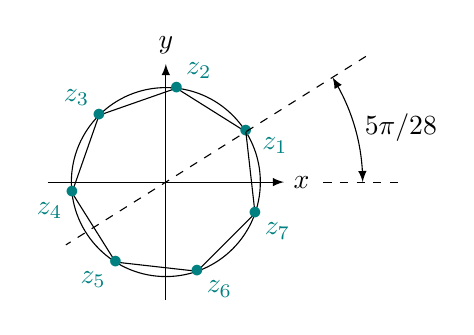
\begin{tikzpicture}
			\draw [-latex] (-1.5, 0) -- (1.5, 0) node [at end, right] {$x$};
			\draw [-latex] (0, -1.5, 0) -- (0, 1.5) node [at end, above] {$y$};
			
			\draw (0,0) circle (1.2cm);
			\foreach \x in {0, 51.428, ..., 308.568} {
				\draw (32.142+\x:1.2) -- (32.142+\x+51.428:1.2);
				\node [teal] at (\x+32.142:1.2) {$\bullet$};
			}
			\node [at={(32.142:1.3)}, teal, below right] {$z_1$};
			\node [at={(32.142 + 51.428:1.2)}, teal, above right] {$z_2$};
			\node [at={(32.142 + 2*51.428:1.2)}, teal, above left] {$z_3$};
			\node [at={(32.142 + 3*51.428:1.2)}, teal, below left] {$z_4$};
			\node [at={(32.142 + 4*51.428:1.2)}, teal, below left] {$z_5$};
			\node [at={(32.142 + 5*51.428:1.2)}, teal, below right] {$z_6$};
			\node [at={(32.142 + 6*51.428:1.2)}, teal, below right] {$z_7$};
			
			\draw [dashed] (32.142:3) -- (180+32.142:1.5);
			\draw [dashed] (2,0)--(3,0);
			\draw [latex-latex] (0:2.5) arc (0:32.142:2.5) node [midway, right] {$5\pi/28$};
		\end{tikzpicture}
	\end{figure}%
	
	% three simple closed domains in the complex plane
	\begin{figure}[h!]\centering
		\begin{subfigure}{0.3\textwidth}
			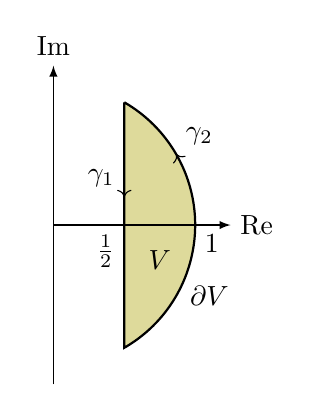
\begin{tikzpicture}[scale=0.9]
				\draw [fill=olive!30, thick]
				(60:2cm)--(-60:2cm) arc (-60:60:2cm)
				;
				\draw[-latex] (0,0)--(2.5,0) 
				node [at end, right] {$\Re$}
				node [at={(2,0)}, below right] {$1$}
				node [at={(1,0)}, below left] {$\frac{1}{2}$};
				
				\draw[-latex] (0,-2.25)--(0,2.25)
				node [at end, above] {$\Im$};
				
				\draw[->] (1,0.5)--(1,0.4)
				node [at end, above left] {$\gamma_1$};
				
				\draw[->] (29:2) arc (29:30:2)
				node [at end, above right] {$\gamma_2$};
				
				\node at (1.5, -0.5) {$V$};
				\node at (2.2, -1) {$\partial V$};
			\end{tikzpicture}
		\end{subfigure}
		\begin{subfigure}{0.3\textwidth}
			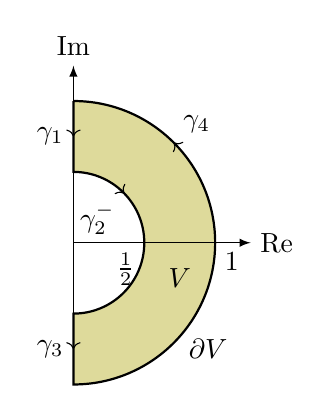
\begin{tikzpicture}[scale=0.9]
				\draw [fill=olive!30, thick]
				(90:2cm)--(90:1cm) arc
				(90:-90:1cm)--(-90:2cm) arc
				(-90:90:2cm)
				;
				\draw[-latex] (0,0)--(2.5,0) 
				node [at end, right] {$\Re$}
				node [at={(2,0)}, below right] {$1$}
				node [at={(1,0)}, below left] {$\frac{1}{2}$};
				
				\draw[-latex] (0,-2)--(0,2.5)
				node [at end, above] {$\Im$};
				
				\draw[->] (0,2)--(0,1.5)
				node [at end, left] {$\gamma_1$};
				
				\draw[->] (45:1) arc (45:44:1)
				node [at end, below left] {$\gamma_2^-$};
				
				\draw[->] (0,-1)--(0,-1.5)
				node [at end, left] {$\gamma_3$};					
				
				\draw[->] (44:2) arc (44:45:2)
				node [at end, above right] {$\gamma_4$};
				
				\node at (1.5, -0.5) {$V$};
				\node at (1.9, -1.5) {$\partial V$};
			\end{tikzpicture}
		\end{subfigure}
		\begin{subfigure}{0.3\textwidth}
			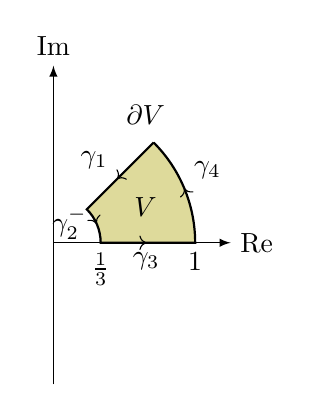
\begin{tikzpicture}[scale=0.9]
				\draw [fill=olive!30, thick]
				(45:2)--(45:2/3) 
				arc (45:0:2/3)--(0:2) 
				arc	(0:45:2)
				;
				\draw[-latex] (0,0)--(2.5,0) 
				node [at end, right] {$\Re$}
				node [at={(2,0)}, below] {$1$}
				node [at={(2/3,0)}, below] {$\frac{1}{3}$};
				
				\draw[-latex] (0,-2)--(0,2.5)
				node [at end, above] {$\Im$};	
				
				\draw[->] (1,1)--(0.9,0.9)
				node [at end, above left] {$\gamma_1$};
				
				\draw[->] (25:2/3) arc (25:24:2/3)
				node [at end, left] {$\gamma_2^-$};
				
				\draw[->] (1.3,0)--(1.31,0)
				node [at end, below] {$\gamma_3$};	
				
				\draw[->] (22:2) arc (22:22.5:2)
				node [at end, above right] {$\gamma_4$};
				
				\node at (1.3, 0.5) {$V$};
				\node at (1.3, 1.8) {$\partial V$};
			\end{tikzpicture}
		\end{subfigure}	    
	\end{figure} %

	%%%%%%%%%%%%%%%%%%%%%%%%%%%%%%%%%%%%%%%%%%%%%%%%%%%%%%%%%%%%%%%%%%%%%%%%%%%%%%%%%%%%%%
	                                 % other drawings %
	%%%%%%%%%%%%%%%%%%%%%%%%%%%%%%%%%%%%%%%%%%%%%%%%%%%%%%%%%%%%%%%%%%%%%%%%%%%%%%%%%%%%%%
	
	% Karnaugh map of a 4-variable minority function.
	\begin{figure}[h!] \centering
		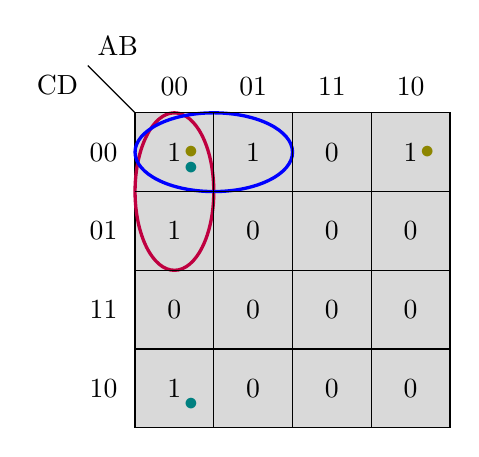
\begin{tikzpicture}
			\draw [fill=gray!30] (0,0) rectangle (4,4);
			\draw (0,4) -- (-0.6,4.6) node [above right] {AB}
			node [below  left] {CD};
			\draw [purple, very thick] (0.5, 3) circle (0.5cm and 1cm);
			\draw [blue, very thick] (1, 3.5) circle (1cm and 0.5cm);
			\foreach \i in {1,2,3,4} {
				\draw (\i, 0) -- (\i, 4) 
				(0, \i) -- (4, \i);
			}  
			
			\path
			(-0.1, 0.5) node [left] {10} ++
			(0,1) node [left] {11} ++
			(0,1) node [left] {01} ++
			(0,1) node [left] {00} ++
			%%
			(0.6, 0.6) node [above] {00} ++
			(1,0) node [above] {01} ++
			(1,0) node [above] {11} ++
			(1,0) node [above] {10}
			%%
			(0.5, 3.5)node{1} node[below right, teal] {$\bullet$} 
			node[right, olive] {$\bullet$}
			++      (1,0) node{1} ++(1,0) node{0} ++(1,0) node {1} node[right, olive] {$\bullet$}
			++  (-3,-1)   node{1} ++(1,0) node{0} ++(1,0) node{0} ++(1,0) node {0}
			++  (-3,-1)   node{0} ++(1,0) node{0} ++(1,0) node{0} ++(1,0) node {0}
			++  (-3,-1)   node{1} node[below right, teal] {$\bullet$}
			++      (1,0) node{0} ++(1,0) node{0} ++(1,0) node {0};
		\end{tikzpicture}
	\end{figure} %
	
	% projection of a function f in L^2 on the vector space V_n. 
	\begin{figure}[h!]\centering
		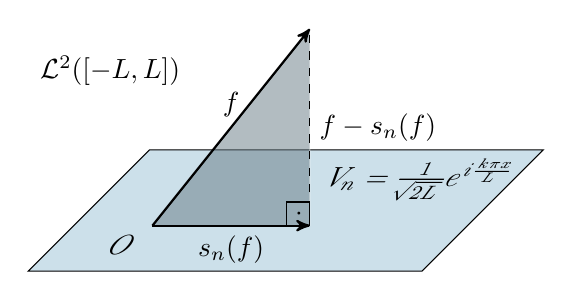
\begin{tikzpicture}[> = stealth']
			\draw [fill=marinho!20] (0,0,0) -- (5,0,0) -- (5,0,4) -- (0,0,4) -- cycle;
			\coordinate (O) at (1,0,2.5);
			\node [at={(O)}, below left, xslant=0.5] {$O$};
			
			\draw [color=white, fill=marinho!20!gray, opacity=0.5] (O) --++ (2,0) --++ (0,2.5) -- cycle;
			
			\draw [->, thick] (O) --++ (2,2.5) node [midway, above] {$f$};
			\draw [->, thick] (O) --++ (2,0) node [midway, below] {$s_n(f)$};
			\draw [dashed] (O) ++ (2,0) --++ (0,2.5) node [midway, right] {$f-s_n(f)$};
			
			\draw (3,0,2.5) rectangle (2.7, 0.3, 2.5);
			\node at (2.86, 0.14, 2.5) {$\cdot$};
			
			\node at (-0.5,1,0) {$\mathcal{L}^2([-L,L])$};
			\node [at={(3.8,0,1)}, xslant=0.5] {$V_n=\frac{1}{\sqrt{2L}}e^{i\frac{k\pi x}{L}}$};
		\end{tikzpicture}
	\end{figure} %
	
	% tresca hexagon and mises ellipse overlapped.
	% here, sigma_e denotes a limitant for the normal tension.
	\begin{figure}[h!]\centering
		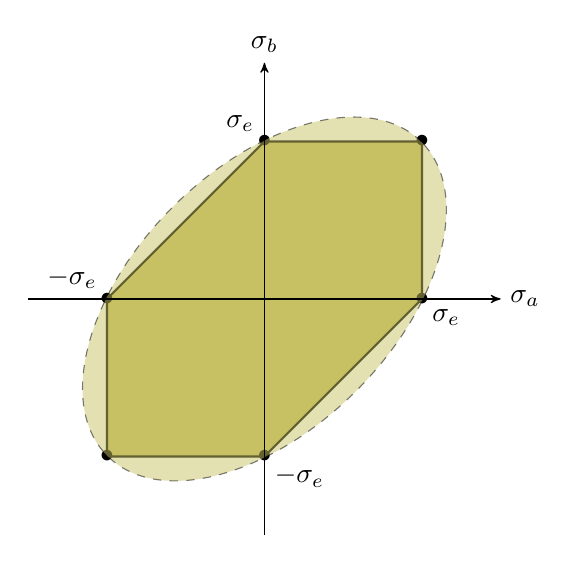
\begin{tikzpicture}[> = stealth']        
			\draw [thick, fill=olive!50] 
			% hexagono
			(0,2) -- (2,2) -- (2,0) -- 
			(0,-2) -- (-2,-2) -- (-2,0) -- cycle
			% casos
			(0, 2) node {$\bullet$}   node [anchor=south east] {$\sigma_e$}
			(2, 2) node {$\bullet$}   
			(2, 0) node {$\bullet$}   node [anchor=north west] {$\sigma_e$}
			(0,-2) node {$\bullet$}  node [anchor=north west] {$-\sigma_e$}
			(-2,-2) node {$\bullet$} 
			(-2, 0) node {$\bullet$}  node [anchor=south east] {$-\sigma_e$}
			;
			
			\begin{scope}[rotate=45]
				\draw [black, fill=olive!50, opacity=0.5, dashed] (0,0) 
				ellipse (2*1.41 and 2*1.41/1.71);
			\end{scope}
			
			\draw [->] (-3,0) -- (3,0) node [right] {$\sigma_a$};
			\draw [->] (0,-3) -- (0,3) node [above] {$\sigma_b$};
		\end{tikzpicture}
	\end{figure} %
	
	% general state of a 3D stress element; 
	% tri-axial state of a 3D stress element;
	% tri-axial state of a 3D stress element cut by a plane pi.
	\begin{figure}[h!] % general state
		\centering
		\begin{subfigure}{0.3\textwidth}
		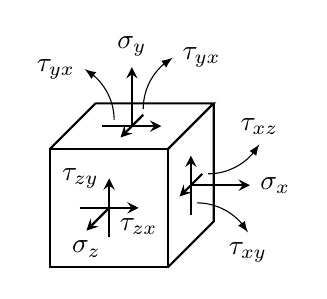
\begin{tikzpicture}[> = stealth, scale=1.5, thick]
			% face frontal
			\draw (0,0,0) -- (1,0,0) -- (1,1,0) -- (0,1,0) -- cycle;
			% face de cima
			\draw (0,1,0) -- (0,1,-1) -- (1,1,-1) -- (1,1,0);
			% face lateral 
			\draw (1,0,0) -- (1,0,-1) -- (1,1,-1);
			
			% tensões na face frontal
			\draw [->] (0.5, 0.25, 0) --++ (0, 0.5) node [anchor=east] {$\tau_{zy}$};
			\draw [->] (0.25, 0.5, 0) --++ (0.5, 0) node [anchor=north] {$\tau_{zx}$};
			\draw [->] (0.5, 0.5, 0) --++ (0,0,0.5) node [anchor=north] {$\sigma_z$};
			
			% tensões na face lateral
			\draw [<-] (1,0.5,-0.25) --++ (0, 0, -0.5);
			\draw [->] (1,0.25, -0.5) --++ (0, 0.5, 0);
			\draw [->] (1, 0.5, -0.5) --++ (0.5, 0, 0) node [anchor=west] {$\sigma_x$};
			
			% tensões na face de cima
			\draw [<-] (0.5, 1, -0.25) --++ (0, 0, -0.5);
			\draw [->] (0.25, 1, -0.5) --++ (0.5, 0, 0);
			\draw [->] (0.5, 1, -0.5) --++ (0, 0.5, 0) node [anchor=south] {$\sigma_y$};
			
			% nomes restantes
			\draw [-latex, thin] (1 +0.05, 0.25 +0.1,-0.5) arc (90:30:0.5) 
			node [anchor=north] {$\tau_{xy}$};
			\draw [-latex, thin] (0.25 +0.1, 1 +0.05, -0.5) arc (0:60:0.5) 
			node [anchor=east] {$\tau_{yx}$};
			\draw [-latex, thin] (1 +0.05, 0.5, -0.75) arc (-90:-30:0.5) 
			node [anchor=south] {$\tau_{xz}$};
			\draw [-latex, thin] (0.5, 1 +0.05, -0.75) arc (180:120:0.5) 
			node [anchor=west] {$\tau_{yx}$};
		\end{tikzpicture}
		\end{subfigure} 
	\hfill
		\begin{subfigure}{0.3\textwidth}
			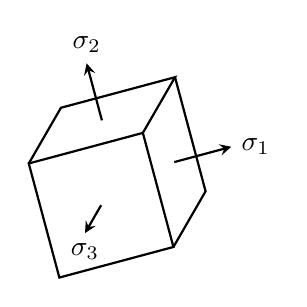
\begin{tikzpicture}[> = stealth, scale=1.5, thick]
				\begin{scope}[rotate=15, shift={(1,0)}]
					% face frontal
					\draw (0,0,0) -- (1,0,0) -- (1,1,0) -- (0,1,0) -- cycle;
					% face de cima
					\draw (0,1,0) -- (0,1,-1) -- (1,1,-1) -- (1,1,0);
					% face lateral 
					\draw (1,0,0) -- (1,0,-1) -- (1,1,-1);
					
					% tensões principais
					\draw [->] (1, 0.5, -0.5) --++ (0.5, 0, 0) node [anchor=west] {$\sigma_1$};
					\draw [->] (0.5, 1, -0.5) --++ (0, 0.5, 0) node [anchor=south] {$\sigma_2$};
					\draw [->] (0.5, 0.5, 0) --++ (0,0,0.5) node [anchor=north] {$\sigma_3$};
				\end{scope}
			\end{tikzpicture}
		\end{subfigure}
	\hfill
		\begin{subfigure}{0.3\textwidth}
			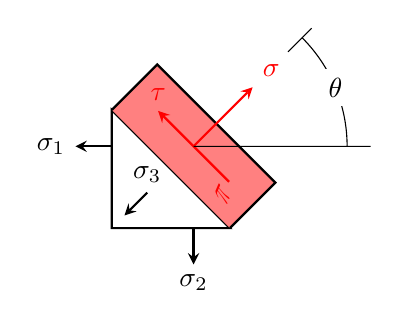
\begin{tikzpicture}[> = stealth, scale=1.5, thick]
				% sigma1, sigma2 
				\draw [->] (0,0.5,-0.5) --++ (-0.5,0,0) node [anchor=east] {$\sigma_1$};
				\draw [->] (0.5,0,-0.5) --++ (0,-0.5,0) node [anchor=north] {$\sigma_2$};
				
				% face triangular 
				\draw [fill=white] (0,0,0) -- (1,0,0) -- (0,1,0) -- cycle;	    
				% face retangular
				\draw [fill=red!50](1,0,0) -- (1,0,-1) -- (0,1,-1) -- (0,1,0);	    
				
				% sigma3
				\draw [->] (0.3, 0.3, 0) node [anchor=south] {$\sigma_3$} --++ (0,0,0.5);
				
				% sigma, tau
				\draw [->, red] (0.5,0.5,-0.5) --++ (0.5, 0.5, 0) 
				node [anchor=south west] {$\sigma$};	 
				\draw [->, red] (0.5,0.5,-0.5) --++ (0.3, -0.3) 
				node [left, xslant=-1, yslant=0.7] {$\pi$} 
				--++ (-0.6,0.6) node [anchor=south] {$\tau$}; 
				
				% theta
				\draw [thin] (0.5,0.5,-0.5) ++ (0.8, 0.8) --++ (0.2,0.2);
				\draw [thin] (0.5,0.5,-0.5) --++ (1.5,0) ++ (-0.2, 0) arc (0:45:1.3) 
				node [midway, fill=white] {$\theta$};
				
			\end{tikzpicture}
		\end{subfigure}
	\end{figure} %

	% Mohr circles defined by the plane pi (see picture above)
	\begin{figure}\centering
		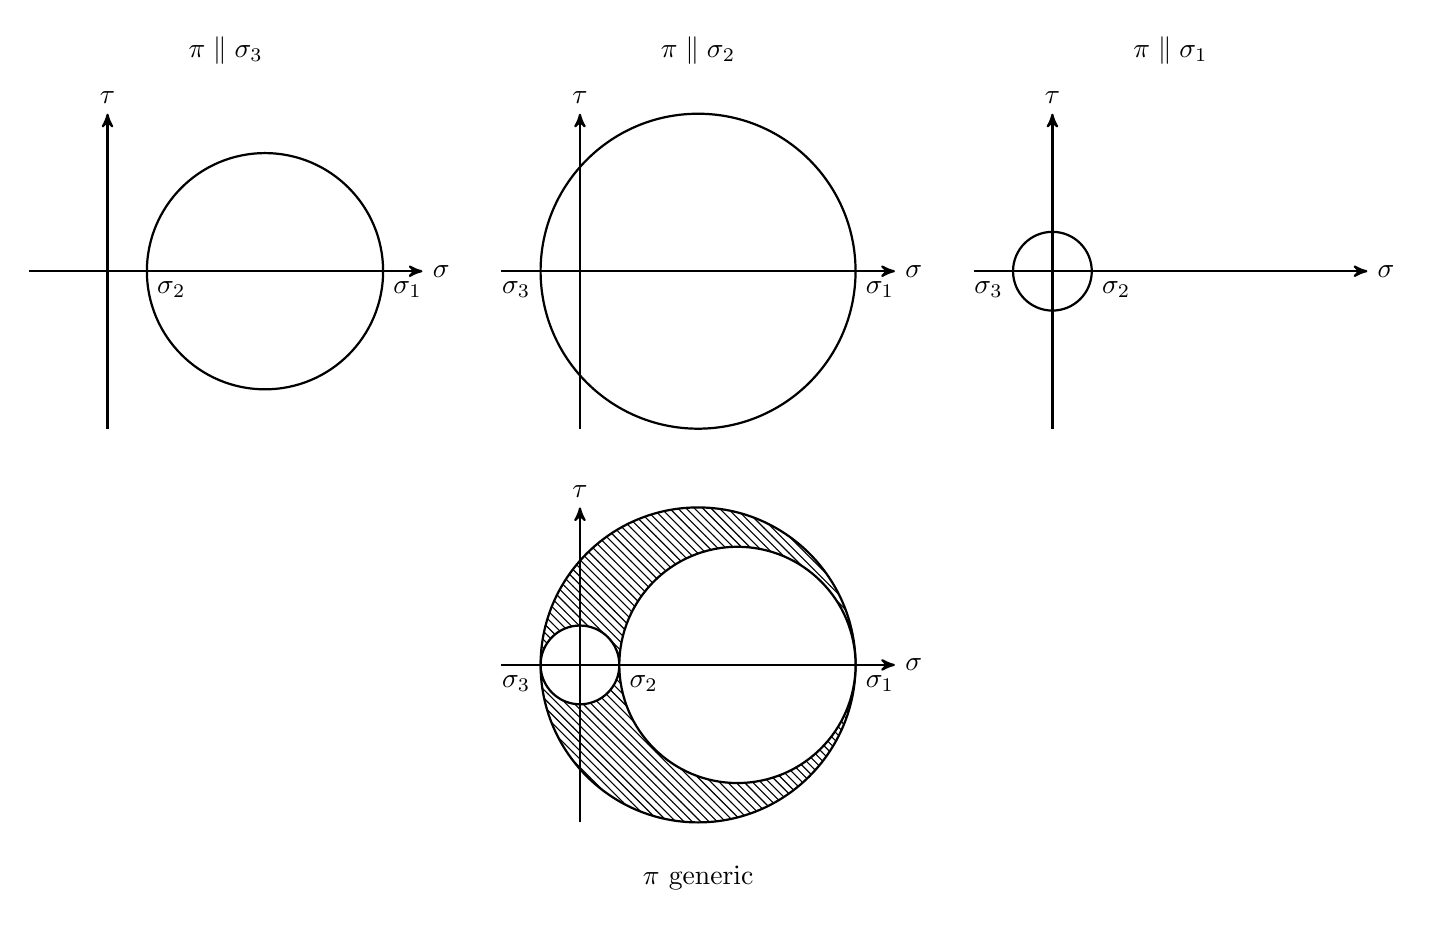
\begin{tikzpicture}[thick, > = stealth']
			% círculo de Mohr pelo eixo 3
			\draw [->] (-1,0) -- (4,0) node [anchor=west] {$\sigma$};
			\draw [->] (0,-2) -- (0,2) node [anchor=south] {$\tau$};
			
			\draw (2,0) circle (1.5)
			(0.5, 0) node [below right] {$\sigma_2$} ++ (3,0) node [below right] {$\sigma_1$};
			
			\node at (1.5, 2.8) {$\pi\parallel\sigma_3$};
			
			% círculo de Mohr pelo eixo 2  
			\begin{scope}[shift={(6,0)}]
				\draw [->] (-1,0) -- (4,0) node [anchor=west] {$\sigma$};
				\draw [->] (0,-2) -- (0,2) node [anchor=south] {$\tau$};
				
				\node at (1.5, 2.8) {$\pi\parallel\sigma_2$};
				
				\draw (1.5,0) circle (2)
				(-0.5, 0) node [below left] {$\sigma_3$} ++ (4,0) node [below right] {$\sigma_1$};	   
				
				% círculo de Mohr pelo eixo 1	  
				\begin{scope}[shift={(6,0)}]
					\draw [->] (-1,0) -- (4,0) node [anchor=west] {$\sigma$};
					\draw [->] (0,-2) -- (0,2) node [anchor=south] {$\tau$};
					
					\draw (0,0) circle (0.5)
					(-0.5, 0) node [below left] {$\sigma_3$} ++ (1,0) 
					node [below right] {$\sigma_2$};
					
					\node at (1.5, 2.8) {$\pi\parallel\sigma_1$};
				\end{scope}
				
				% junção de todos
				\begin{scope}[shift={(0,-5)}]	       
					\draw [pattern = north west lines] (1.5,0) circle (2);
					\draw [fill=white] (0,0) circle (0.5)	 
					(2,0) circle (1.5)
					(-0.5, 0) node [below left] {$\sigma_3$} ++ (1,0) node [below right] {$\sigma_2$} 
					++ (3,0) node [below right] {$\sigma_1$};
					
					\draw [->] (-1,0) -- (4,0) node [anchor=west] {$\sigma$};
					\draw [->] (0,-2) -- (0,2) node [anchor=south] {$\tau$};
					
					\node at (1.5, -2.7) {$\pi$ generic};
				\end{scope}
			\end{scope}	  
		\end{tikzpicture}
	\end{figure} %
	
	% trajectory curve s and hodograph path h of a particle. 
	\begin{figure}[h!] % trajectory
		\centering
		\begin{subfigure}{0.4\textwidth}\centering
			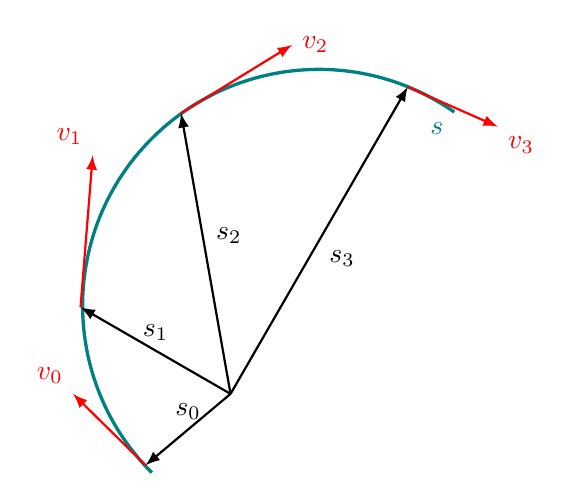
\begin{tikzpicture}
				%% Trajetória s
				\draw [very thick, teal] (-1,-1) arc (225:55:3)
				node [at end, below left] {$s$};
				
				%% Alguns vetores s de s
				\draw [-latex, thick] (0,0)--(220:1.41)
				node [midway, above] {$s_0$};
				
				\draw [-latex, thick] (0,0)--(150:2.2)
				node [midway, above] {$s_1$};
				
				\draw [-latex, thick] (0,0)--(100:3.62)
				node [midway, above right] {$s_2$};
				
				\draw [-latex, thick] (0,0)--(60:4.5)
				node [midway, below right] {$s_3$};
				
				%% Alguns vetores v de s
				\draw [-latex, red, thick] (220:1.41)--(180:2)
				node [at end, above left] {$v_0$};
				
				\draw [-latex, red, thick] (150:2.2)--(120:3.5)
				node [at end, above left] {$v_1$};
				
				\draw [-latex, red, thick] (100:3.62)--(80:4.5)
				node [at end, right] {$v_2$};
				
				\draw [-latex, red, thick] (60:4.5)--(45:4.8)
				node [at end, below right] {$v_3$};			  
			\end{tikzpicture}
		\end{subfigure}
		\hfill
		\begin{subfigure}{0.4\textwidth} % hodograph
			\centering
			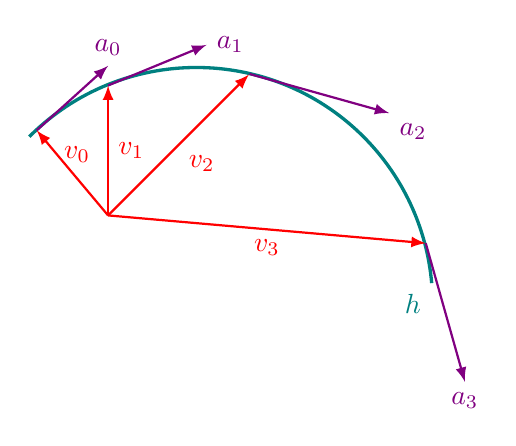
\begin{tikzpicture}
				%% Hodógrafa
				\draw [very thick, teal] (-1,1) arc (135:5:3)
				node [at end, below left] {$h$};
				
				%% Vetores v da hodógrafa
				\draw [-latex, thick, red] (0,0)--(130:1.41)
				node [midway, above] {$\,\,v_0$};
				
				\draw [-latex, thick, red] (0,0)--(90:1.65)
				node [midway, right] {$v_1$};
				
				\draw [-latex, thick, red] (0,0)--(45:2.53)
				node [midway, below right] {$v_2$};
				
				\draw[-latex, thick, red] (0,0)--(-5:4.05)
				node [midway, below] {$v_3$};
				
				%% Vetores a da hodógrafa
				\draw[-latex, thick, violet] (130:1.41)--(90:1.9)
				node [at end, above] {$a_0$};
				
				\draw[-latex, thick, violet] (90:1.65)--(60:2.5)
				node [at end, right] {$a_1$};
				
				\draw[-latex, thick, violet] (45:2.54)--(20:3.8)
				node [at end, below right] {$a_2$};
				
				\draw[-latex, thick, violet] (-5:4.05)--(-25:5)
				node [at end, below] {$a_3$};	
				
			\end{tikzpicture}\vspace{0.7cm}
			\caption*{A hodógrafa \color{teal}$h$ \color{black} de uma partícula.\\
				É uma abstração.}
		\end{subfigure}
	\end{figure} %
	
	% 'polka dotted' diagram in which a point (n,m) simbolizes the result of a_n*b_m. 
	\begin{figure}[h!]\centering
		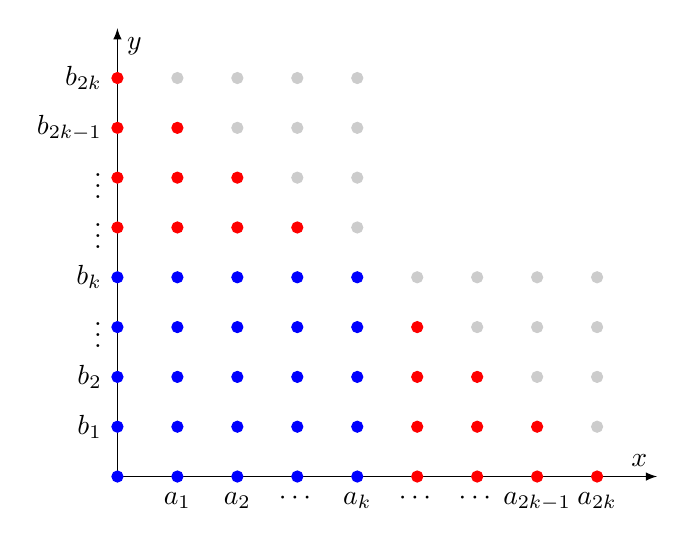
\begin{tikzpicture}
			\begin{axis}[
				axis x line = middle,    	 
				axis y line = middle,     
				axis line style = {-latex},
				xmin=0, xmax=9, ymin=0, ymax=9,
				xlabel = {$x$},		
				xtick = {1,...,8},
				xticklabels = 
				{$a_1$, $a_2$, $\cdots$, $a_k$, $\cdots$, $\cdots$,$a_{2k-1}$, $a_{2k}$},
				ylabel = {$y$},
				ytick = {1,...,8},
				yticklabels = 
				{$b_1$, $b_2$, $\vdots$, $b_k$, $\vdots$, $\vdots$,$b_{2k-1}$, $b_{2k}$}
				]
				%% Quadrado azul
				\addplot [bluedot] 
				coordinates{ 					
					(0,0) (0,1) (0,2) (0,3) (0,4) 
					(1,0) (1,1) (1,2) (1,3) (1,4) 
					(2,0) (2,1) (2,2) (2,3) (2,4) 
					(3,0) (3,1) (3,2) (3,3) (3,4) 
					(4,0) (4,1) (4,2) (4,3) (4,4)  					 				
				};
				
				\addplot [reddot]
				coordinates{
					%% Triangulo vermelho superior
					(3,5)
					(2,5) (2,6)
					(1,5) (1,6) (1,7)
					(0,5) (0,6) (0,7) (0,8)	 				
					%% Triangulo vermelho inferior  
					(8,0)  	 
					(7,0) (7,1)  
					(6,0) (6,1) (6,2) 	
					(5,0) (5,1) (5,2) (5,3)
				};
				
				\addplot [graydot]
				coordinates{
					(1,8) 
					(2,8) (2,7)
					(3,8) (3,7) (3,6)
					(4,8) (4,7) (4,6) (4,5)
					%%
					(8,1) 
					(8,2) (7,2)
					(8,3) (7,3) (6,3)
					(8,4) (7,4) (6,4) (5,4)
				};
			\end{axis}
		\end{tikzpicture}
	\end{figure} %
	
	% intersection of intervals on the real line.
	\begin{figure}[h!]\centering
		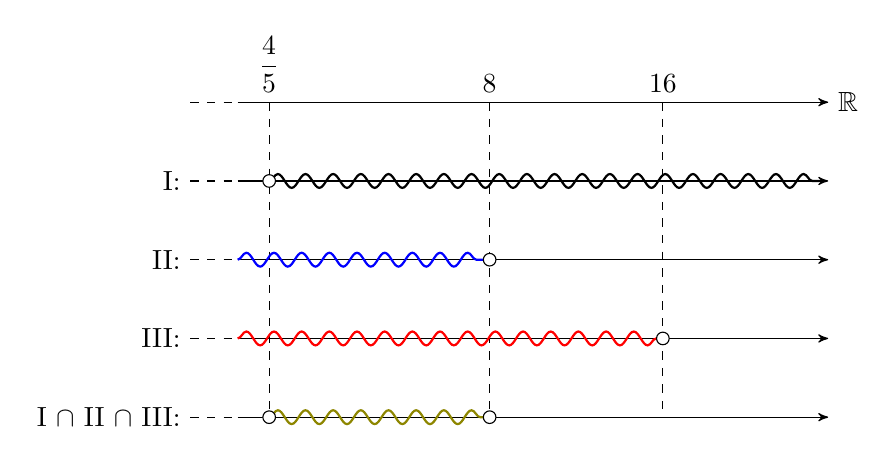
\begin{tikzpicture}[> = stealth',
			decoration = {snake}]
			\draw[dashed] (0,0) --++ (0.6, 0)
			(0,-1) --++ (0.6, 0)
			(0,-2) --++ (0.6, 0)
			(0,-3) --++ (0.6, 0)
			(0,-4) --++ (0.6, 0)
			%
			(1,0) node [above] {$\displaystyle{\frac{4}{5}}$} --++ (0,-4)
			(3.8,0) node [above] {$8$} --++ (0,-4)
			(6,0) node [above] {$16$} --++ (0,-4)
			%
			(0,-1) node [anchor=east] {I:}
			(0,-2) node [anchor=east] {II:}
			(0,-3) node [anchor=east] {III:}
			(0,-4) node [anchor=east] {I $\cap$ II $\cap$ III:}
			;
			
			\draw[->] (0.6,0) -- (8.1,0) node [right] {$\mathbb{R}$};
			\draw[->] (0.6,-1) -- (8.1,-1);
			\draw[->] (0.6,-2) -- (8.1,-2);
			\draw[->] (0.6,-3) -- (8.1,-3);
			\draw[->] (0.6,-4) -- (8.1,-4);
			
			\path[draw, decorate, thick] (1, -1) -- (8,-1);
			\path[draw, decorate, thick, blue] (0.6, -2) -- (3.8,-2);
			\path[draw, decorate, thick, red] (0.6, -3) -- (6,-3);
			\path[draw, decorate, thick, olive] (1, -4) -- (3.8,-4);
			
			\draw[fill=white] 
			(1, -1) circle (0.08)
			(3.8, -2) circle (0.08)
			(6, -3) circle (0.08)
			(1, -4) circle (0.08)
			(3.8, -4) circle (0.08);
		\end{tikzpicture}
	\end{figure} %
	
	% handy diagram for remembering the vector product between the unit vectors i, j, and k.
	\begin{figure}
		\centering
		\begin{subfigure}{0.2\textwidth}
			% follow the arrows for a positive result, e.g., i x j = +k.
			\begin{tikzpicture}
				\coordinate[label=below:$\ihat$] (I) at (0,1.732);				
				\coordinate[label=$\jhat$] (J) at (-1,0);
				\coordinate[label=$\khat$] (K) at (1,0);
				
				\coordinate (X) at (1,2);
				\coordinate (Y) at (-1,2);
				\coordinate (Z) at (-0.5,0.5);
				\coordinate (V) at (0.5,0.5);
				\coordinate (U) at (0,1.9);
				
				\draw pic["", draw=black, ->, angle eccentricity=1.3, angle radius=1.9cm]{angle=Y--K--Z};
				
				\draw pic["", draw=black, ->, angle eccentricity=1.3, angle radius=1.9cm]{angle=V--J--X};
				
				\draw pic["+", draw=black, ->, angle eccentricity=1.3, angle radius=1.9cm]{angle=Z--U--V};
			\end{tikzpicture}
		\end{subfigure}
		\hspace{1cm}
		\begin{subfigure}{0.2\textwidth}
			% follow the arrows for a negative result, e.g., j x i = -k.
			\begin{tikzpicture}
				\coordinate[label=below:$\ihat$] (I) at (0,1.732);				
				\coordinate[label=$\jhat$] (J) at (-1,0);
				\coordinate[label=$\khat$] (K) at (1,0);
				
				\coordinate (X) at (1,2);
				\coordinate (Y) at (-1,2);
				\coordinate (Z) at (-0.5,0.5);
				\coordinate (V) at (0.5,0.5);
				\coordinate (U) at (0,1.9);
				
				\draw pic["", draw=black, <-, angle eccentricity=1.3, angle radius=1.9cm]{angle=Y--K--Z};
				
				\draw pic["", draw=black, <-, angle eccentricity=1.3, angle radius=1.9cm]{angle=V--J--X};
				
				\draw pic["--", draw=black, <-, angle eccentricity=1.3, angle radius=1.9cm]{angle=Z--U--V};
			\end{tikzpicture}
		\end{subfigure}
	\end{figure} %

	% Mohr circle of a 2D stress element
	\begin{figure}[h!]\centering
		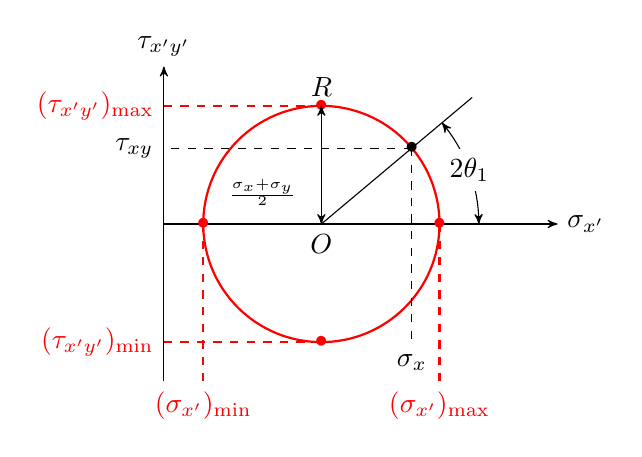
\begin{tikzpicture}[> = stealth']
			\draw [->] (0, 0) -- (5,0) node [right] {$\sigma_{x'}$};
			\draw [->] (0,-2) -- (0,2) node [above] {$\tau_{x'y'}$};
			
			\draw [red, thick] (2,0) node [black, below] {$O$} circle (1.5cm);                          
			
			\draw [red, thick, dashed] (2, 1.5) node {{\small$\bullet$}} -- (0, 1.5) 
			node [left] {$(\tau_{x'y'})_\text{max}$};       
			
			\draw [red, thick, dashed] (2,-1.5) node {{\small$\bullet$}} -- (0,-1.5) 
			node [left] {$(\tau_{x'y'})_\text{min}$};
			
			\draw [red, thick, dashed] (0.5, 0) node {{\small$\bullet$}}
			--++ (0,-2) node [below] {$(\sigma_{x'})_\text{min}$};
			\draw [red, thick, dashed] (3.5, 0) node {{\small$\bullet$}}
			--++ (0,-2) node [below] {$(\sigma_{x'})_\text{max}$};
			
			\draw [<->] (2,0) --++ (0, 1.5) node [above] {$R$}; 
			\node at (1.25,0.4) {{\tiny$\frac{\sigma_x+\sigma_y}{2}$}};    
			
			\draw [dashed] (2,0) ++ (40:1.5) node {{\small$\bullet$}} --++ (-3.16,0)
			node [left] {$\tau_{xy}$}; 
			\draw [dashed] (2,0) ++ (40:1.5) --++ (0,-2.5) node [below] {$\sigma_x$};
			
			\draw (2,0) --++ (40:2.5);
			\draw [<->] (4,0) arc (0:40:2) node [midway, fill=white] {$2\theta_1$};
		\end{tikzpicture}
	\end{figure} %
	
\end{document}